\documentclass[11pt,a4paper,titlepage]{article}
\usepackage[utf8]{inputenc}
\usepackage{amsmath}
\usepackage{amsfonts}
\usepackage{csvsimple}
\usepackage{amssymb}
\usepackage{hyperref}
\hypersetup{
    colorlinks=true,
    linkcolor=black,
    filecolor=black,
    urlcolor=cyan,
    citecolor=black,
}

\usepackage{tikz}
\usetikzlibrary{calc,patterns,angles,quotes,shapes.geometric, arrows}

\def\layersep{2.5cm}


\tikzstyle{train} = [rectangle, rounded corners, minimum width=2.2cm, minimum height=1cm,text centered, draw=black, fill=red!30]
\tikzstyle{test} = [rectangle, rounded corners, minimum width=2.2cm, minimum height=1cm,text centered, draw=black, fill=green!30]
\tikzstyle{data} = [rectangle, rounded corners, minimum width=11.8cm, minimum height=1cm,text centered, draw=black, fill=gray!30]
\tikzstyle{MSE} = [rectangle, rounded corners, minimum width=1.4cm, minimum height=1cm,text centered, draw=black, fill=orange!30]
\tikzstyle{arrow} = [thick,->,>=stealth]

\usepackage{float}
%\usepackage{mathtools}
\usepackage{bm}
\usepackage[margin=1in]{geometry}

\title{Project 2 in FYS-STK4155}
\author{Adrian Martinsen Kleven & Simon Elias Schrader }
\date{Autumn 2020}
\usepackage{hyperref}

\usepackage{natbib}
\usepackage{graphicx}
\graphicspath{{../figures/presentable_data/}} %Setting the graphicspath

\begin{document}
%\maketitle
\tableofcontents
\listoffigures
\listoftables

\clearpage
\section{Abstract}
Machine learning - is it possible to learn this power? - Anakin\\
Strong in you The computational power is! - Yoda\\
It doesn't converge! This is outrageous! This is unfair! How can you call something machine learning but don't learn nothing at all? - Anakin\\
Meesa computer master now! - Jar Jar Binks\\
Hello np.where()! - Obi Wan Kenobi\\
INFINITE CONVERGENCE - The senate
\section{Introduction}
As can be seen in \citep{Project1}, both Ordinary Least Square (OLS) regression and  Ridge regression failed to accurately fit a polynomial function to geographic data and did not manage to match the surface properly. In this article, we analyse whether regression with the help of feed forward neural networks (FFNNs) can give better results (in the form of a lower Mean Square Error) than OLS and Ridge regression. In order to do so, we implemented several stochastic gradient methods to find the approximate minimum of the Mean Square Error (MSE) function in parameter space. In order to evaluate their quality, we first compared their performance to the analytical expressions for OLS and Ridge regression for several parameters. Later, these methods were used in the back propagation of the neural network. For the regression problem, we used the sigmoid function as well as RELU and LeakyRELU as activation functions for the hidden layers and the linear function for the output layer. We did this comparison for several stochastic gradient methods and a flexible number of hidden layers and neutrons per hidden layer. \\
We also tested the neural network's performance on a categorization problem, namely the MNIST data set \citep{lecun2010mnist}. We compared several activation functions for the hidden layers, while using the Softmax function (or the sigmoid function) for the output layer. Finally, we compared the neural network's performance to the results achieved using logistic regression. \\
In this report, we will first describe the methods used, focusing on stochastic gradient descent methods and the theory of FFNNs. This is done in the method part. The result part cointains 
\section{Methods}
\subsection{Logistic Regression}
Logistic regression is a regression algorithm applied to binary classification problems. A weighted and biased sum of predictors are passed through the logistic activation function and a cost function is applied to the output and the accompanying label to the set of predictors. The problem of finding the weights and biases that predict the correct category then becomes a problem of optimizing the cost function by tweaking the weights and biases. Logistic regression is in many ways comparable to linear regression. The key difference arises in the use of the Logistic or Softmax activation function.
\begin{figure}[H]
\begin{center}
\begin{tikzpicture}
  \draw[->] (-4, 0) -- (4, 0) node[right] {$x$};
  \draw[dashed] (-4, 1) -- (4, 1)node[above] {$y=1$} ;
  \draw[->] (0, -0.5) -- (0, 1.5) node[above] {$y$};
  \draw[scale=1, domain=-4:4, smooth, variable=\x, blue] plot ({\x}, {1/(1+e^(-\x))});
\end{tikzpicture}
\end{center}
\caption[Logistic function]{The logistic function outputs a number between $0$ and $1$ for every function input.}
\label{logisticfunc}
\end{figure}
The logistic function, seen in figure \ref{logisticfunc} naturally translates a range of inputs into a probability distribution of two outcomes.
\paragraph{Multinomial logistic regression} is the generalization of logistic regression to multi- class problems and uses the Softmax activation function. We will consider multinomial logistic regression from here on, as the Softmax function reduces to the logistic function in the case where the number of categories is 2 (\ref{ProofSoftmaxToLogistic}).\\\\Given a dataset of $L$ datapoints, $N$ predictors and $m$ categories, we structure the dataset thus
\begin{equation}\label{first}
\textbf{X} = 
\begin{pmatrix}
	x_{1,1} &	x_{1,2}	&	\cdots	&	x_{1,N}	\\
	x_{2,1}	&	x_{2,2}	&	\cdots	&	x_{2,N}	\\
	\vdots	&	\vdots	&	\cdots	&	\vdots	\\
	x_{L,1} &	x_{L,1}	&	\cdots	&	x_{L,N}	
\end{pmatrix}\,\,\,\,\textbf{Y} = 
\begin{pmatrix}
	y_{1,1} &	y_{1,2}	&	\cdots	&	y_{1,m}	\\
	y_{2,1}	&	y_{2,2}	&	\cdots	&	y_{2,m}	\\
	\vdots	&	\vdots	&	\cdots	&	\vdots	\\
	y
	_{L,1} &	y_{L,1}	&	\cdots	&	y_{L,m}	
\end{pmatrix}
\end{equation}
Where $\textbf{X}$ is a $L\times N$ matrix with the predictors corresponding to a datapoint arranged along the row. $\textbf{Y}$ a $L\times m$ matrix wherein every row of the matrix is a vector in the One- hot representation corresponding to the label describing the datapoint in the corresponding row in $\textbf{X}$.\\ The weights are arranged in a $m \times N$ matrix and the biases in a $m \times 1$ vector
\begin{equation}
\textbf{W} = \begin{pmatrix}
	w_{1,1} &	w_{1,2}	&	\cdots	&	w_{1,N}	\\
	w_{2,1}	&	w_{2,2}	&	\cdots	&	w_{2,N}	\\
	\vdots	&	\vdots	&	\cdots	&	\vdots	\\
	w_{m,1} &	w_{m,1}	&	\cdots	&	w_{m,N}	
\end{pmatrix}\,\, , \,\, \textbf{b} = 
\begin{pmatrix}
	b_1	\\
	b_2	\\
	\vdots	\\
	b_m
\end{pmatrix}.
\end{equation}
The weighted sum for a datapoint $l$ is then given by 
\begin{equation}
\textbf{z}^{(l)} = \textbf{W}\textbf{x}^{(l)}+\textbf{b} \textit{ where }\textbf{x}^{(l)}=(\textbf{X}_{[l,:]})^T
\end{equation}
and the $i'th$ activation by
\begin{equation}\label{softmax}
a_i^{(l)} = \frac{e^{z_i^{(l)}}}{\sum_{j=1}^{m} e^{z_j^{(l)}}}.
\end{equation}
Given that the labels are structured in the One- hot representation, the cross- entropy cost function for a single datapoint $l$ is given by
\begin{equation}\label{last}
C^{(l)} = \sum\limits_{j=1}^{m} -y_j^{(l)}\log(a_i^{(l)}).
\end{equation}
The algorithm can be understood as a single layer perceptron with $m$ neurons in the hidden layer. In figure \ref{LogisticRegressionDiagram} below, the functions and variables in the nodes are as given in equations \eqref{first} to \eqref{last}.

\begin{figure}[H]


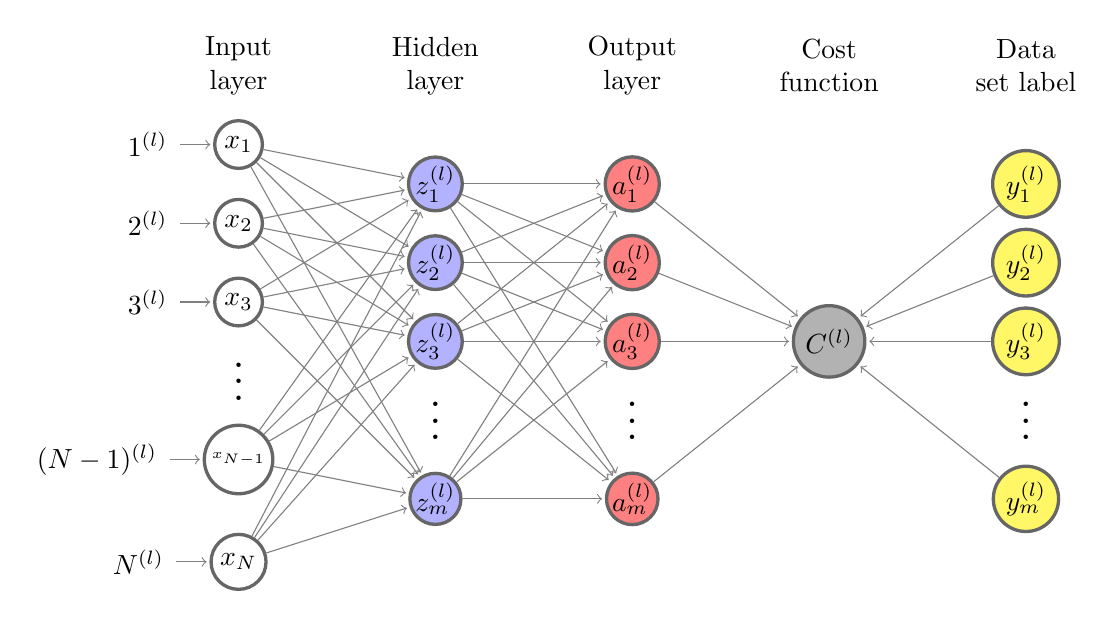
\begin{tikzpicture}[shorten >=1pt,->,draw=black!50, node distance=\layersep]
    \tikzstyle{every pin edge}=[<-,shorten <=1pt]
    \tikzstyle{neuron}=[circle,draw=black!60,fill=black!25,minimum size=17pt,inner sep=0pt, very thick]
    \tikzstyle{missing}=[draw=none, scale=1.5,text height=0.333cm,execute at begin node=\color{black}$\vdots$]
    \tikzstyle{input neuron}=[neuron, fill=white!50,inner sep=2pt];
    \tikzstyle{output neuron}=[neuron, fill=red!50];
    \tikzstyle{hidden neuron}=[neuron, fill=blue!30];
    \tikzstyle{cost neuron}=[neuron, fill=black!30,inner sep=2.4pt];
    \tikzstyle{label neuron}=[neuron, fill=yellow!60,inner sep=1.6pt];
    \tikzstyle{annot} = [text width=4em, text centered]

    % Draw the input layer nodes
    \foreach \name / \y in {1,2,3}
    	\path[yshift=0.5cm]
        	node[input neuron, pin=left:$\y^{(l)}$] (I-\name) at (0,-\y) {$x_\y$};
    \path[yshift=0.5cm]
    	node[missing] (I-4) at (0,-4) {};
    \path[yshift=0.5cm]
		node[input neuron, pin=left:$(N-1)^{(l)}$] (I-5) at (0,-5) {\tiny $x_{N-1}$};
	\path[yshift=0.2cm]
    	node[input neuron, pin=left:$N^{(l)}$] (I-6) at (0,-6) {$x_{N}$};
    
    % Draw the hidden layer nodes
    
    \foreach \name / \y in {1,2,3}
        \path[yshift=0.0cm]
            node[hidden neuron] (H-\name) at (\layersep,-\y cm) {$z_\y^{(l)}$};
    
    \path[yshift=0.0cm]
            node[missing] (H-4) at (\layersep,-4 cm) {};
    
    \path[yshift=0.0cm]
            node[hidden neuron] (H-5) at (\layersep,-5 cm) {$z_m^{(l)}$};

    % Draw the output layer
    
    \foreach \name / \y in {1,2,3}
        \path[yshift=0.0cm]
            node[output neuron] (O-\name) at (2*\layersep,-\y cm) {$a_\y^{(l)}$};
    
    \path[yshift=0.0cm]
            node[missing] (O-4) at (2*\layersep,-4 cm) {};
    
    \path[yshift=0.0cm]
            node[output neuron] (O-5) at (2*\layersep,-5 cm) {$a_m^{(l)}$};
            
     % Draw the Cost node
    
    \node[cost neuron, right of=O-3] (C) {$C^{(l)}$};
    
    % Draw the label layer
    
    \foreach \name / \y in {1,2,3}
        \path[yshift=0.0cm]
            node[label neuron] (Y-\name) at (4*\layersep,-\y cm) {$y_\y^{(l)}$};
    
    \path[yshift=0.0cm]
            node[missing] (Y-4) at (4*\layersep,-4 cm) {};
    
    \path[yshift=0.0cm]
            node[label neuron] (Y-5) at (4*\layersep,-5 cm) {$y_m^{(l)}$};


    % Connect every node in the input layer with every node in the
    % hidden layer.
    \foreach \source in {1,2,3,5,6}
        \foreach \dest in {1,2,3,5}
            \path (I-\source) edge (H-\dest);
	
    
    % Connect every node in the hidden layer with the output layer
    \foreach \source in {1,2,3,5}
        \foreach \dest in {1,2,3,5}
            \path (H-\source) edge (O-\dest);
	
	% Connect every node in the Output layer with the Cost node
    \foreach \source in {1,2,3,5}
        \path (O-\source) edge (C);	
	
	% Connect every node in the label layer with the Cost node
    \foreach \source in {1,2,3,5}
            \path (Y-\source) edge (C);	
	
    % Annotate the layers
    \node[annot,above of=I-1, node distance=1cm] (i1) {Input layer};
    \node[annot,right of=i1, node distance=\layersep] (hl) {Hidden layer};
    \node[annot,right of=hl, node distance=\layersep] (o1) {Output layer};
    \node[annot,right of=o1, node distance=\layersep] (c1) {Cost function};
    \node[annot,right of=c1, node distance=\layersep] (y1) {Data set label};
\end{tikzpicture}
\caption[Logistic regression diagram]{The single layer perceptron model of multinomial logistic regression.}
\label{LogisticRegressionDiagram}
\end{figure}
\subsubsection{Cost function}
In stochastic gradient descent, the cost function we will end up using in the below calculations are given by 
\begin{equation}
C = \sum\limits_{l=1}^{Batch\,size} C^{(l)}
\end{equation}
\subsubsection{Derivatives of the cost function}
We want to calculate the derivative of the new cost function with respect to the weights and biases. We will use these to calculate the step in the gradient descent:
$\textbf{W} = \textbf{W} -\eta \frac{d C}{d\textbf{W} }$ and $\textbf{b} = \textbf{b} -\eta \frac{d C}{d\textbf{b} }$. Using the chain rule, we can re-express this problem as
\begin{equation}\label{backprop1}
\frac{dC}{dw_{i,n}} = \sum_{j=1}^m \left (\frac{dC}{da_j} \right) \left (\frac{da_j}{dz_i} \right) \left(\frac{dz_i}{dw_{i,n}} \right )
\end{equation}
and
\begin{equation}\label{backprop2}
\frac{dC}{db_i} = \sum_{j=1}^m \left (\frac{dC}{da_j} \right) \left (\frac{da_j}{dz_i} \right) \left(\frac{dz_i}{db_i} \right )
\end{equation}
where $i \in [1,2,\cdots,m]$ and $n \in [1,2,\cdots,N]$. We can now proceed to solving each of these derivatives in turn:
\begin{equation}
\frac{dC^{(l)}}{da_j^{(l)}} = - \frac{y_j^{(l)}}{a_j^{(l)}},\,\,\, \frac{dz_i^{(l)}}{dw_{i,n}^{(l)}} =  x_n^{(l)},\,\,\, \frac{dz_i^{(l)}}{db_i^{(l)}} =  1.
\end{equation}
The derivative of the Softmax function $$\frac{da_j^{(l)}}{dz_i^{(l)}}$$ is $$a_j^{(l)}(\delta_{ji}-a^{(l)}_i)$$ but rather than this expression, we want to formulate the derivative as a $m \times m$ matrix:
\begin{equation}
\frac{d}{d \textbf{z}^{(l)}} \textbf{a}^{(l)} = (\textbf{a}^{(l)} \otimes \mathbf{1} )\circ (\mathbf{I} - \mathbf{1} \otimes \textbf{a}^{(l)}) = \textbf{M}
\end{equation}
where $\mathbf{1}$ is the $m \times 1$ one- vector, $ \mathbf{I} $ is the $m \times m$ unit matrix, $\otimes$ is the outer product and $\circ$ is the Hadamard product. The reason for this seemingly convoluted change in perspective, becomes apparent when we consider our equations \eqref{backprop1} and \eqref{backprop2}, which are now expressible (for a single datapoint) as
\begin{equation}
\frac{dC^{(l)}}{d\textbf{W}} =  \textbf{M}\cdot(- \textbf{y}^{(l)}\oslash \textbf{a}^{(l)}) \textbf{x}^{(l)}
\end{equation}
and
\begin{equation}
\frac{dC^{(l)}}{d\textbf{b}} =  \textbf{M}\cdot(- \textbf{y}^{(l)}\oslash \textbf{a}^{(l)}) 
\end{equation}
where $\oslash$ is the Hadamard division. With the gradients in hand, we can now optimize the weights and biases through gradient descent.

\subsubsection{Algorithm}
The algorithm for Logistic regression goes as follows. We make an initial guess for the weights and biases. Using these and a data point we calculate the activation function. This is then used, together with the same data point in calculating the gradient of the cost function, which is used to calculate the new, optimized parameters $\textbf{W}$ and $\textbf{b}$.
\begin{figure}[H]
\begin{center}
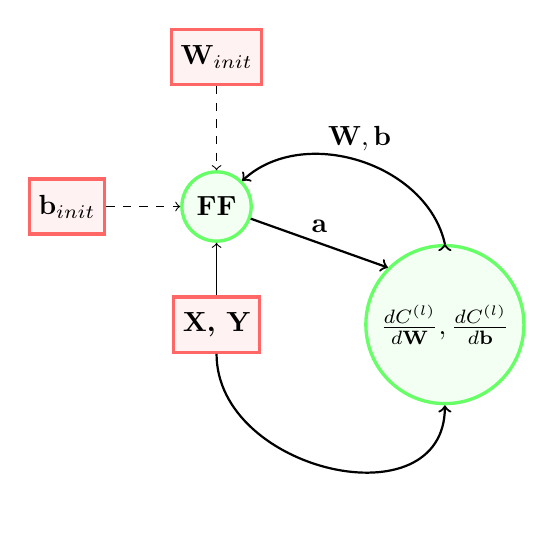
\begin{tikzpicture}[
roundnode/.style={circle, draw=green!60, fill=green!5, very thick, minimum size=7mm},
squarednode/.style={rectangle, draw=red!60, fill=red!5, very thick, minimum size=7mm},]
%Nodes
\node[squarednode]      (Winit)                              {$\textbf{W}_{init}$};
\node[roundnode, yshift = -0.9cm]      (FF)  [below of = Winit]{$\textbf{FF}$};
\node[squarednode, xshift = -0.9cm]      (binit)  [left of = FF]{$\textbf{b}_{init}$};
\node[squarednode, yshift = -0.5cm]      (XY)  [below of = FF]{$\textbf{X, Y}$};
\node[roundnode, xshift = 1.9cm]      (grad)  [right of = XY]{$\frac{dC^{(l)}}{d\textbf{W}},\frac{dC^{(l)}}{d\textbf{b}}$};

%Lines
\draw[->,dashed] (Winit.south) -- (FF.north);
\draw[->,dashed] (binit.east) -- (FF.west);
\draw[->] (XY.north) -- (FF.south);

\path[->,draw,thick] (FF) edge node[above] {$\textbf{a}$} (grad.north west);

\draw[->,thick] (XY.south) .. controls +(down:15mm) and +(down:15mm) .. (grad.south);

\path[->,draw,thick] (grad.north) edge [bend right=60] node[above] {$\textbf{W},\textbf{b}$} (FF.north east);
\end{tikzpicture}
\end{center}
\caption[Logistic regression algorithm]{The algorithmic structure of logistic regression. Red squares represent variables that enter the algorithm. Green circles represent computations and dashed arrows means the output is used once.}
\label{LogisticRegressionDiagram}
\end{figure}
This process continues until either a given number of iterations have taken place, or the Softmax function produces an output error within a given tolerance. 
\subsection{Gradient Descent Methods}
One way to find the minima, both local and global, of a (multivariable) function, one can use the method of gradient descent. Simply speaking, this is done by iteratively changing the parameters in order to minimize a cost function \citep{handsOnMachineLearning}. As the gradient of a function always shows towards the point of steepest descent, following the gradient in the opposite direction will lead to a minimum. In both regression and classification problems, the function to be minimized is the cost function. In terms of linear regression, the cost function is the MSE function (possibly with additional regularization). The gradient is simply a vector containing the partial derivatives with respect to each coefficient $\beta_i$.\\
For OLS and Ridge regression, we have that 
\begin{equation}
     \nabla_\beta C(\beta)=\frac{2}{m} \left[X^T \left(X\beta-y\right)\textcolor{red}{+\lambda\beta} \right]
\end{equation}
where C is the cost function, X is the design matrix and m is the number of inputs. The \textcolor{red}{red} part is only added for Ridge Regression. \\
After having an initial guess for the values $\beta^0$, The values $\beta$ are then be updated iteratively by following the gradient in the opposite direction:
\begin{equation}\label{Updatescheme}
\beta^{i+1}=\beta^{i}- \gamma \nabla_\beta C(\beta^{i})
\end{equation}
where we introduced the learning rate $\gamma$. The learning rate $\gamma$ needs to be chosen in such a way that it is not too large (which can lead to divergent behaviour), but not too small either (which can lead to an extremely slow convergence). This is done either until convergence is reached, or for a given number of iterations, called \textit{epochs}.
\subsubsection{Stochastic Gradient Descent Methods}
Because calculating the gradient of every parameter $\beta$ can be rather costly for large data sets, the gradient can be approximated by the gradient at only one input variable which is chosen randomly. This introduces randomness and erratic behaviour to the way the minimum is found. It is hence likely that the minimum is well approximated, but not exact \citep{handsOnMachineLearning}. However, the advantage is that the stochastic method can "jump out of" local minima and find the global minimum. One closely related method is Mini-batch gradient descent, where the gradient is approximated by the gradient at several, but not all, randomly chosen input variables. This leads to a less erratic behaviour, but is still computationally cheaper than Gradient Descent.
There are several ways to implement the actual gradient descent. It is useful to adapt the learning rate $\gamma$ as the program proceeds - starting with a comparatively large learning rate, the algorithm can  leave local minima and proceed to the global minimum, while the learning rate is gradually reduced to get better convergence. In the following, three methods of varying complexity will be introduced.
\paragraph*{"Naive" Stochastic Gradient Descent} has a constant learning rate $\gamma$, and the parameters $\beta$ are just updated by \eqref{Updatescheme} where the gradient is approximated. While this is easy to implement, has only one parameter ($\gamma$) to be fine tuned, and is cheap to calculate, the non-adaptive learning rate $\gamma$ can lead to sub-optimal convergence.
\paragraph*{Decaying $\gamma$}
- A simple way to make $\gamma$ get smaller gradually is to implement a gradual decay. Defining
\begin{equation}
\gamma_t=\frac{t_0}{t_1+t}
\end{equation}
where $t_0$ and $t_1$ are initialization parameters and t is updated as $t=e\cdot m+i$ where $e$ is the actual epoch, $i$ is the actual mini batch and $m$ is the number of mini batches. The update scheme remains the same \eqref{Updatescheme}, just that $\gamma_t$ is used instead of a fixed $\gamma$. While this method has the advantage that $\gamma_t$ gradually gets reduced, eventually $\gamma$ gets so small that the steplength gets so small that no convergence is reached.
\paragraph*{RMSProp} describes a method where the learning rate is reduced gradually by accumulating the gradients from previous iterations, however, unlike the previous method, the impact of previous iterations decays exponentially. The update scheme is described as 
\begin{equation}
\begin{split}
    &\bm{s}^{i+1}=\alpha \bm{s}^{i}+(1-\alpha) \nabla_\beta C(\bm{\beta^{i}})* \nabla_\beta C(\bm{\beta^{i}}) \\
   &\bm{\beta}^{i+1}=\bm{\beta}^{i}-\gamma C(\bm{\beta^{i}}) / \sqrt{\bm{s}^{i+1}+e}
\end{split}
\end{equation}
where * and / refer to element-wise multiplication and division, respectively. In this article, we chose the default value $\alpha=0.9$, while $e=10^{-8}$ simply has the purpose of avoiding zero division.
\paragraph*{ADAM} is a method related to RMSProp, and is a shortcut for \textit{adaptive momentum estimation}. It combines features of RMSProp and a method called Momentum optimization (see for example \citep{MortenLectureNotes}) - it keeps track of the average of past gradients, but also the average of past gradients squared, and both are to decay exponentially. The update scheme is described as 
\begin{equation}
\begin{split}
    & \bm{m}^{i+1}=[\alpha_1\bm{m}+(1-\alpha_1) \nabla_\beta C(\bm{\beta^{i}})](1-\alpha_1^T)^{-1}\\
    &\bm{s}^{i+1}=\alpha_2 \bm{s}^{i}+(1-\alpha_2) \nabla_\beta C(\bm{\beta^{i}})* \nabla_\beta C(\bm{\beta^{i}})(1-\alpha_2^T)^{-1} \\
   &\bm{\beta}^{i+1}=\bm{\beta}^{i}-\gamma\bm{m}^{i+1} / \sqrt{\bm{s}^{i+1}+e}
\end{split}
\end{equation}
where * and /  again refer to element-wise multiplication and division, respectively; and T stands for the number of iterations (starting at 1). In this article, we chose the default values $\alpha_1=0.9$ and $\alpha_2=0.99$, while $e=10^{-8}$ simply has the purpose of avoiding zero division.
\subsection{Neural networks}
\subsubsection{Feed forward?}
\subsubsection{Back propagation}
\subsubsection{Activation functions}
As described in the previous to subsections, the activation function is one of the core elements in Neural Networks. In this project, we implemented the following four activation functions for activation between the input layer and the first hidden layer as well as between all hidden layers. For the output, we used no activation function (Regression) or the Softmax activation function (Classification). 

\paragraph*{sigmoid function} - The sigmoid function, defined as $\sigma(x)=\frac{e^x}{e^x-1}$, outputs function values between 0 and 1 for all inputs. It is inspired by the way Neurons fire in the brain [XXX].
\paragraph*{tanh} - The tanh function, which can be expressed in terms of the sigmoid function $tanh(x)=2\sigma(2x)-1$, can take functions between -1 and 1. Unlike the sigmoid function, it maps negative inputs to negative function values, while 0 is mapped to 0.
\paragraph*{ReLU} -The ReLU function (\textit{Rectified Linear Unit}) is defined as $ReLU(x)=x^+$ (x if x is positive, zero otherwise). Unlike the tanh function and the sigmoid function, it does not suffer from vanishing gradients when the input values are large. It has been shown \citep{surpremeRELU} that rectifiers can give better results in Machine learning, especially depper networks, than the sigmoidal functions.
\paragraph*{LeakyReLU} - The LeakyReLU function is defined as $LeakyReLU(x)=max(x,\alpha x)$ where $\alpha=0.01$ (though other values are possible, too). Positive values are hence mapped to themselves, whereas negative input values are mapped to $\alpha x$. Unlike the ReLU function, it has nonzero output for negative input values too, and the gradient vanishes nowhere, improving the problem of "dying" neurons.
\subsection{Data sets}
\subsubsection{Regression: Geographic Data}
For the regression analysis, we used the same data as in \citep{Project1} - a black-and white image with resolution $3601 \times 3601$ pixel which represents an area in the Taebaek Mountains in South Korea with a total surface area of $3601 \times 3601km^2$ , hence each square kilometer is represented as one pixel, where colour intensity represents the height (black equals height at sea level).
\subsubsection{Classification: MNIST data set}
For classification, we use the MNIST data set, a data set consisting of 70.000 handwritten digits between 0 and 9, represented as a picture with resolution $28\times28$ pixel \citep{lecun2010mnist}. In this article however we used Scikit Learn's variant of the MNIST data set, which consists of 1797 elements with resolution $8\times8$ pixel. 
\section{Computational implementation}

\subsection{Multinomial logistic regression}


\subsubsection{Numerically stable variants}
The Softmax function defined in \eqref{softmax}, is inherently prone to overflow. We can resolve this by making a small change:
\begin{equation}
a_i= \frac{e^{z_i}}{\sum_{j=1}^{m} e^{z_j}} \cdot \frac{e^{-c}}{e^{-c}}
\end{equation}


\subsection{Neural network}
\subsubsection{Setting up weights and biases for the neural network}
As there is no clear rule how to set up weights and biases, other than that they should be initialized with a non-zero value, we first tried to set up the weights with a mean zero normal distribution with a small standard deviation $\sigma\approx0.01$. However, we found that this yielded undesirable results, which made that especially ReLU and LeakyReLU gave unpredictable behaviour where the activation function gave very high numbers, eventually leading to numerical instability and overflow. Hence, we decided to follow the approach described in \cite{DelvingDeep}, where the weights are initialized randomly, following a mean zero normal distribution with standard deviation $\sigma=\sqrt{2/n\_inputs}$ where n\_inputs here refers to the batch size. The biases were simply initialized with a small nonzero number - $0.001$.
\subsubsection{Functionality of the Neural Network}
We designed a flexible Neural Network that works with any amount of hidden layers and any amount of neurons per hidden layer. It works with both classification and regression, using the softmax function as activation function for the output layer for classification, and simply the linear function $f(x)=x$ for the regression case. 
\section{Results}
\subsection{Comparison of SGD methods for OLS}
Figure \ref{fig:DifferentSGD} shows, for a given OLS problem, the test MSE as a function of the learning rate $\eta$ for a fixed number of epochs \& a fixed batch size; the test MSE as a function of the number of epochs for a fixed learning rate \& a fixed batch size; and the test MSE as a function of batch size for a fixed number of epochs and a fixed learning rate. 

\begin{figure}[H]
\centering
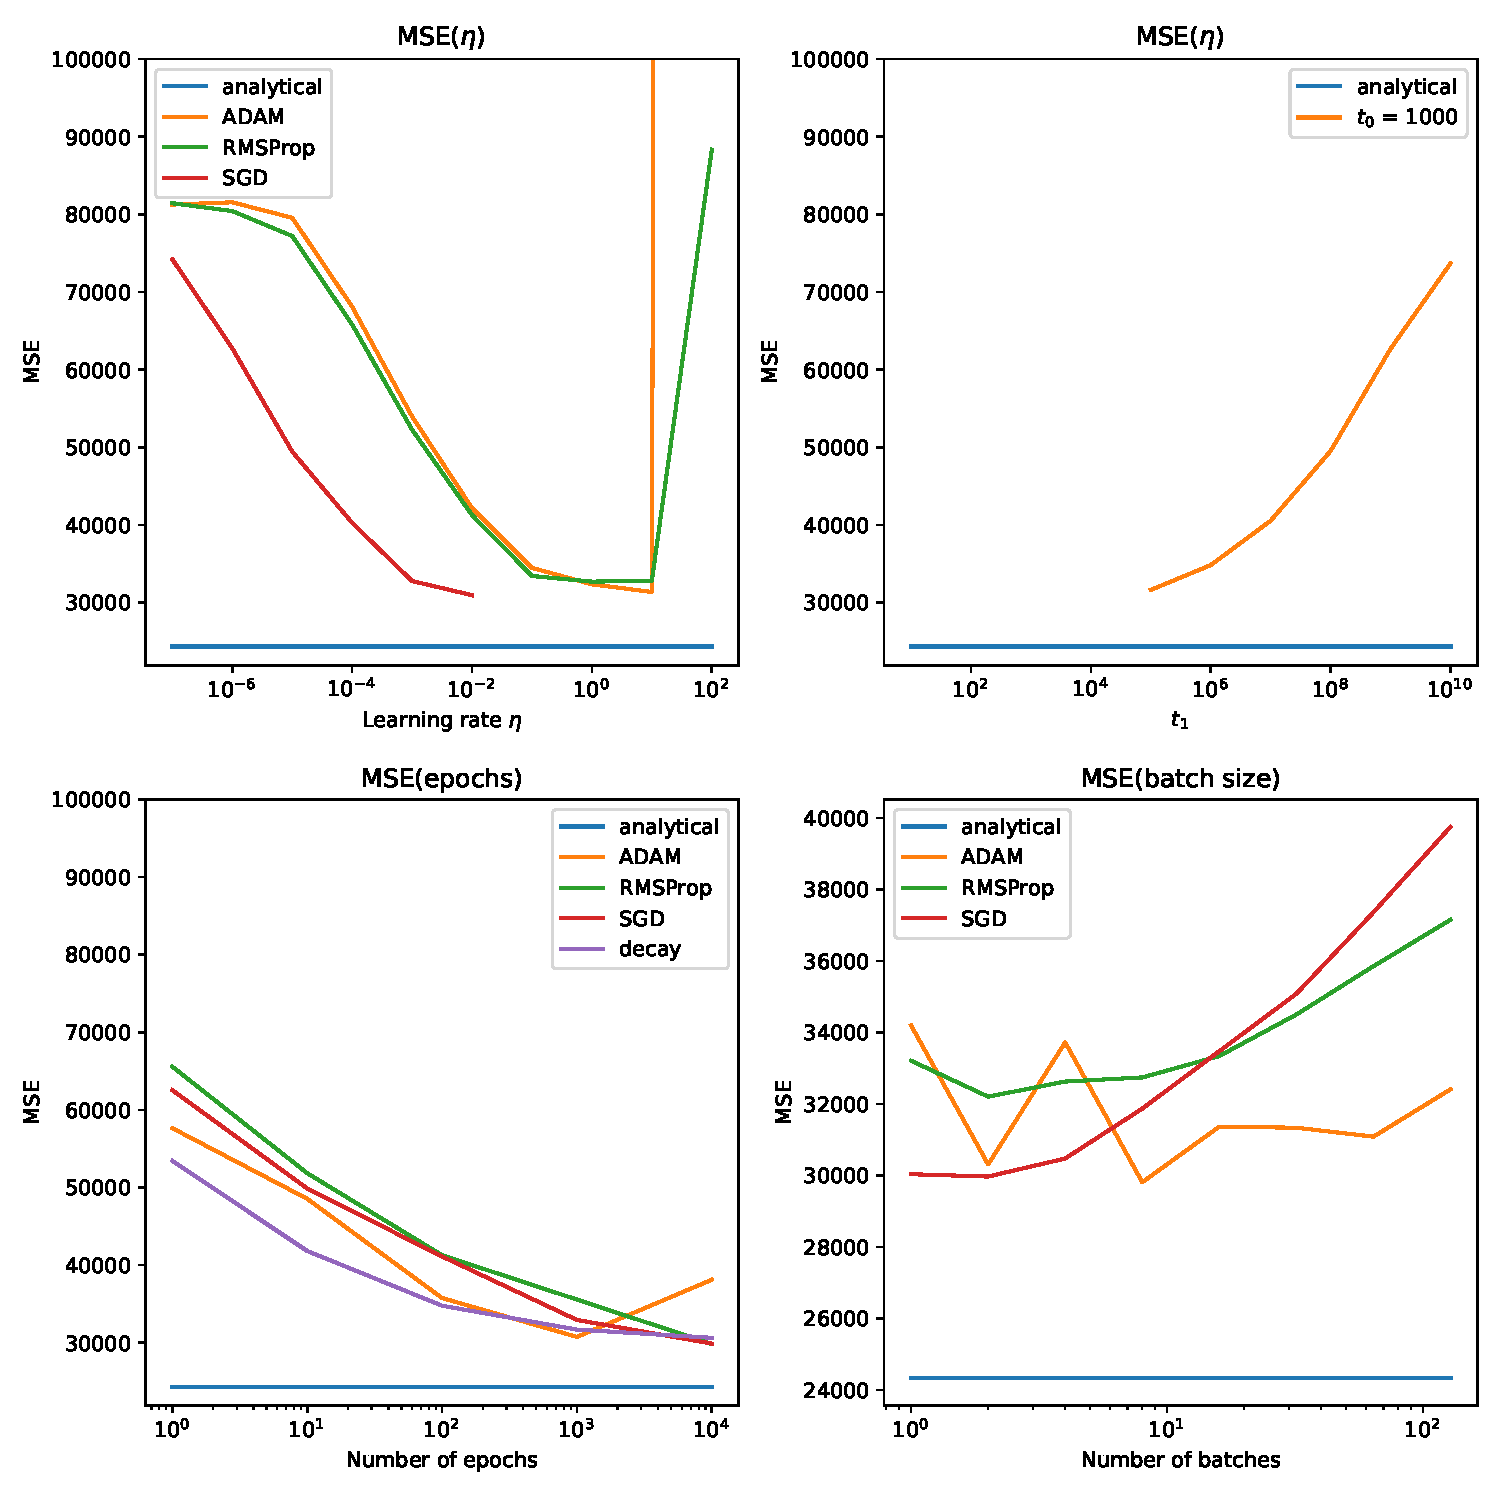
\includegraphics[width=0.95\textwidth]{OLS_error_SGD_idealLearningRate.pdf}
\caption[Test MSE Different SGD methods for OLS]{The simple SGD method (titled SGD), RMSProp, ADAM and decaying $\eta$ as functions of the learning rate $\eta$ (top left), the number $t_1$ (top right), the number of epochs (down left), and different batch sizes (down right). The number of data points is $N=2000$, the polynomial degree used is $deg=10$. For the top two plots, a batch size of 16 and and epoch of 1000 were chosen. The lower to plots use the ideal parameters $\eta$ and $t_1$ which were chosen based on the ideal values from first two plots. No bootstrapping or cross-validation was performed.}\label{fig:DifferentSGD}
\end{figure}
As one can see, the number of epochs and the learning rate make a huge difference when it comes to approximating the analytical solution. For the decay-SGD and the simple SGD (titled SGD), the curves are truncated because too big or too small values lead to NaN-values. This shows that the ideal learning rate is dangerously close to a too high learning rate, leading to completely wrong numbers or even NaN-values. Similar observations can be done for both ADAM and RMSProp, but the change is not as drastic for these methods.\\ 
As expected, the number of epochs lead to increased error reduction for all methods. However, even though the number of epochs grows exponentially, the error reduction slows down and even ceases. This is hence a computationally expensive way of reducing the extra error. As the learning rate was chosen to be ideal for 1000 epochs, we also see that, at least with ADAM, the error actually increases - this might be due to over-fitting, or leaving the reached minimum.\\
The number of batches does not seem to have a large impact on the quality of the fit for  ADAM, but we observe that the simple SGD method and RMSProp work best with small batch sizes. This might be because these methods work best when making many "small hops" instead of several larger hops.\\
One can see that the choice of method has a large impact on how fast the error is reduced. RMSProp and ADAM seem to be slightly superior to the simple SGD in terms of convergence to the true MSE, however their biggest advantage is that they are more stable and have "broader" ideal learning rates. This is not surprising as these methods were developed for this purpose. ADAM seems to be better at dealing with higher epochs than RMSProp though. The decay-fit method, while giving results as good as RMSProp and ADAM for ideal parameters, is too unstable to be used in practice - small fluctuations in the parameters lead to completely wrong values. It is also harder to tweak several parameters. 
Figure \ref{fig:DifferentSGD_fixedEta} contains the same plots as figure \ref{fig:DifferentSGD}, however, the learning rates $\eta$ were chosen so that they didn't exceed a value of 0.1. This is more difficult to do for the decay method, which we left unchanged. One can see that this leads to a slightly different behaviour. The convergence is, not surprisingly, slower, but the methods behave slightly less erratic. That way, the error keeps reducing as the number of epochs increases, but it takes more epochs to get it to the same level as before. Also, the error now increases for larger batch sizes for all methods, including ADAM. In this implementation, a larger batch size has no computational advantages, however, for the Neural Network later, larger batch sizes give increased run time. 
\begin{figure}[H]
\centering
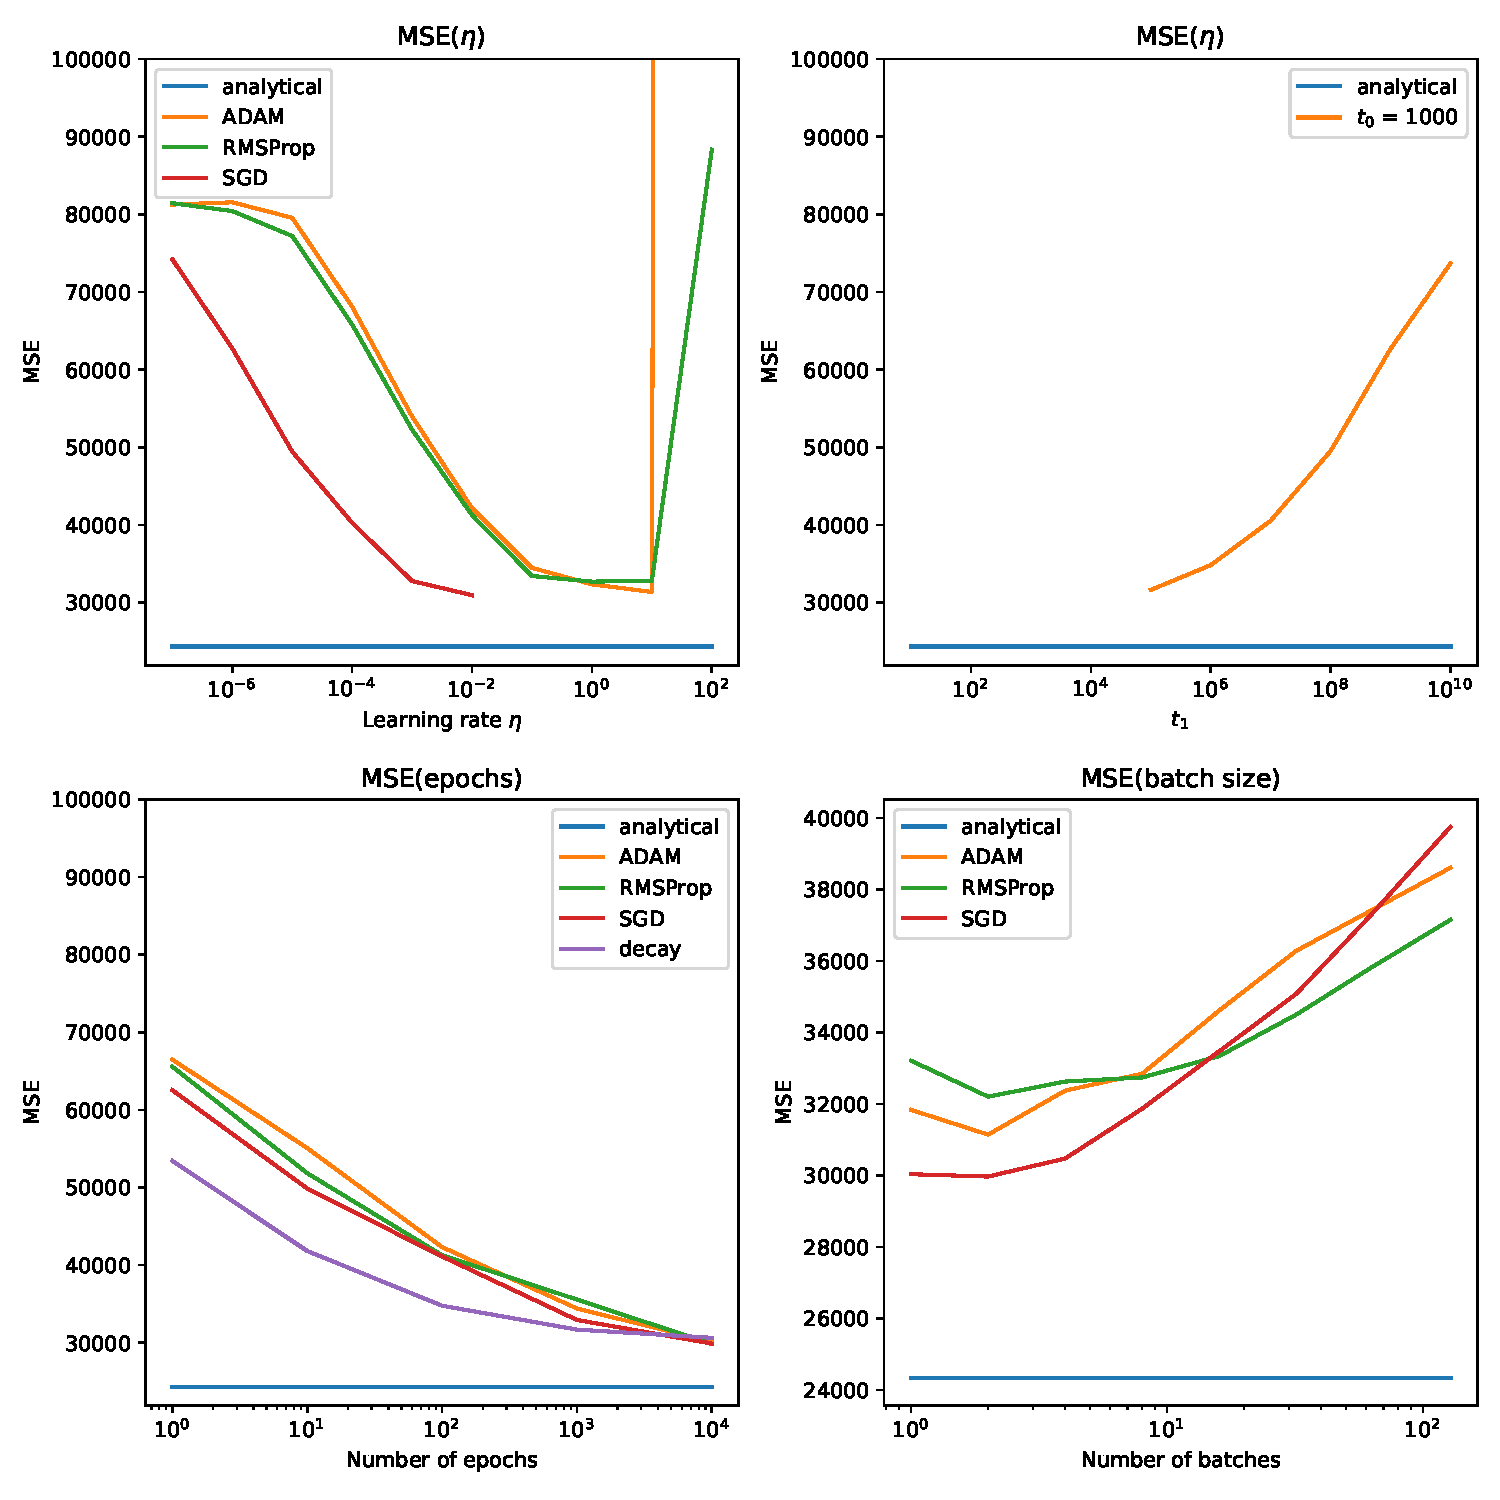
\includegraphics[width=0.95\textwidth]{OLS_error_SGD_fixedLearningRate.pdf}
\caption[Test MSE Different SGD methods for OLS (fixed $\eta$)]{The simple SGD method (titled SGD), RMSProp, ADAM and decaying $\eta$ as functions of the learning rate $\eta$ (top left), the number $t_1$ (top right), the number of epochs (down left), and different batch sizes (down right). The number of data points is $N=2000$, the polynomial degree used is $deg=10$. For the top two plots, a batch size of 16 and and epoch of 1000 were chosen. The lower to plots use the ideal parameters $\eta$ and $t_1$ which were chosen based on the first two plots, however, $\eta$ was chosen so that $\eta \leq 0.1$ as larger numbers lead to instability later on. No bootstrapping or cross-validation was performed.}\label{fig:DifferentSGD_fixedEta}
\end{figure}
\subsubsection{Comparison of SGD methods for Ridge regression}
We repeated the same analysis as above with Ridge regression, only varying the learning rate and the regularisation parameter, keeping the batchsize fixed (16), as well as the number of epochs (1000). We chose a high polynomial degree where OLS is inferior to Ridge regression. The results can be seen in figure \ref{fig:DifferentSGDRIDE} in the appendix. The difference between the methods is baffling. We see that simple SGD gives NaN-values for too high learning rates, as before. RMSProp and ADAM, too, give worse results as the learning rate increases, but to a much lesser degree than simple SGD. As we did not perform Cross Validation, these numbers are only qualitatively correct, but we see that all methods, given the ideal parameters are chosen, can get very close to the analytical result. ADAM performs best and manages to come close to the analytical solution, however, both RMSProp and the simple SGD method get quite close, too. We see that regularization gives improved values for Stochastic Gradient Descent methods, to, as very small regularization parameters $\lambda$ yield worse test errors than the optimal parameters. We see however that the error is always larger than the ideal test error, implying that Stochastic Gradient Descent methods can get quite close, but not exactly equal to the ideal analytical parameters, at least not with the chosen parameters. 
\subsection{FFNN for Regression}
We used randomly selected points from the geographic data \citep{Project1} to create a fit using both OLS and Ridge Regression, as well as the Neural Network.
\subsubsection{Comparing the FFNN to Scikit-learn}
We tested the quality of our Neural Network with N=2000 randomly selected data points and a polynomial degree of 10. We chose 200 as batch size and 1000 epochs. We used one hidden layer with 100 neurons. The sigmoid function was used as activation function for the hidden layer, and simple gradient descent was used. Figure \ref{fig:ScikitLearn_1} plots the test and train error as function of the regularization parameter $\lambda$ and the error learning rate $\eta$. Using OLS, we found 28272 for the test MSE and 24758 for the train MSE, for comparison. We also compared this to Scikit-learn 's MLPRegressor function \citep{scikit-learn}, which are included in figure \ref{fig:ScikitLearn_1}.
\begin{figure}[H]
\centering
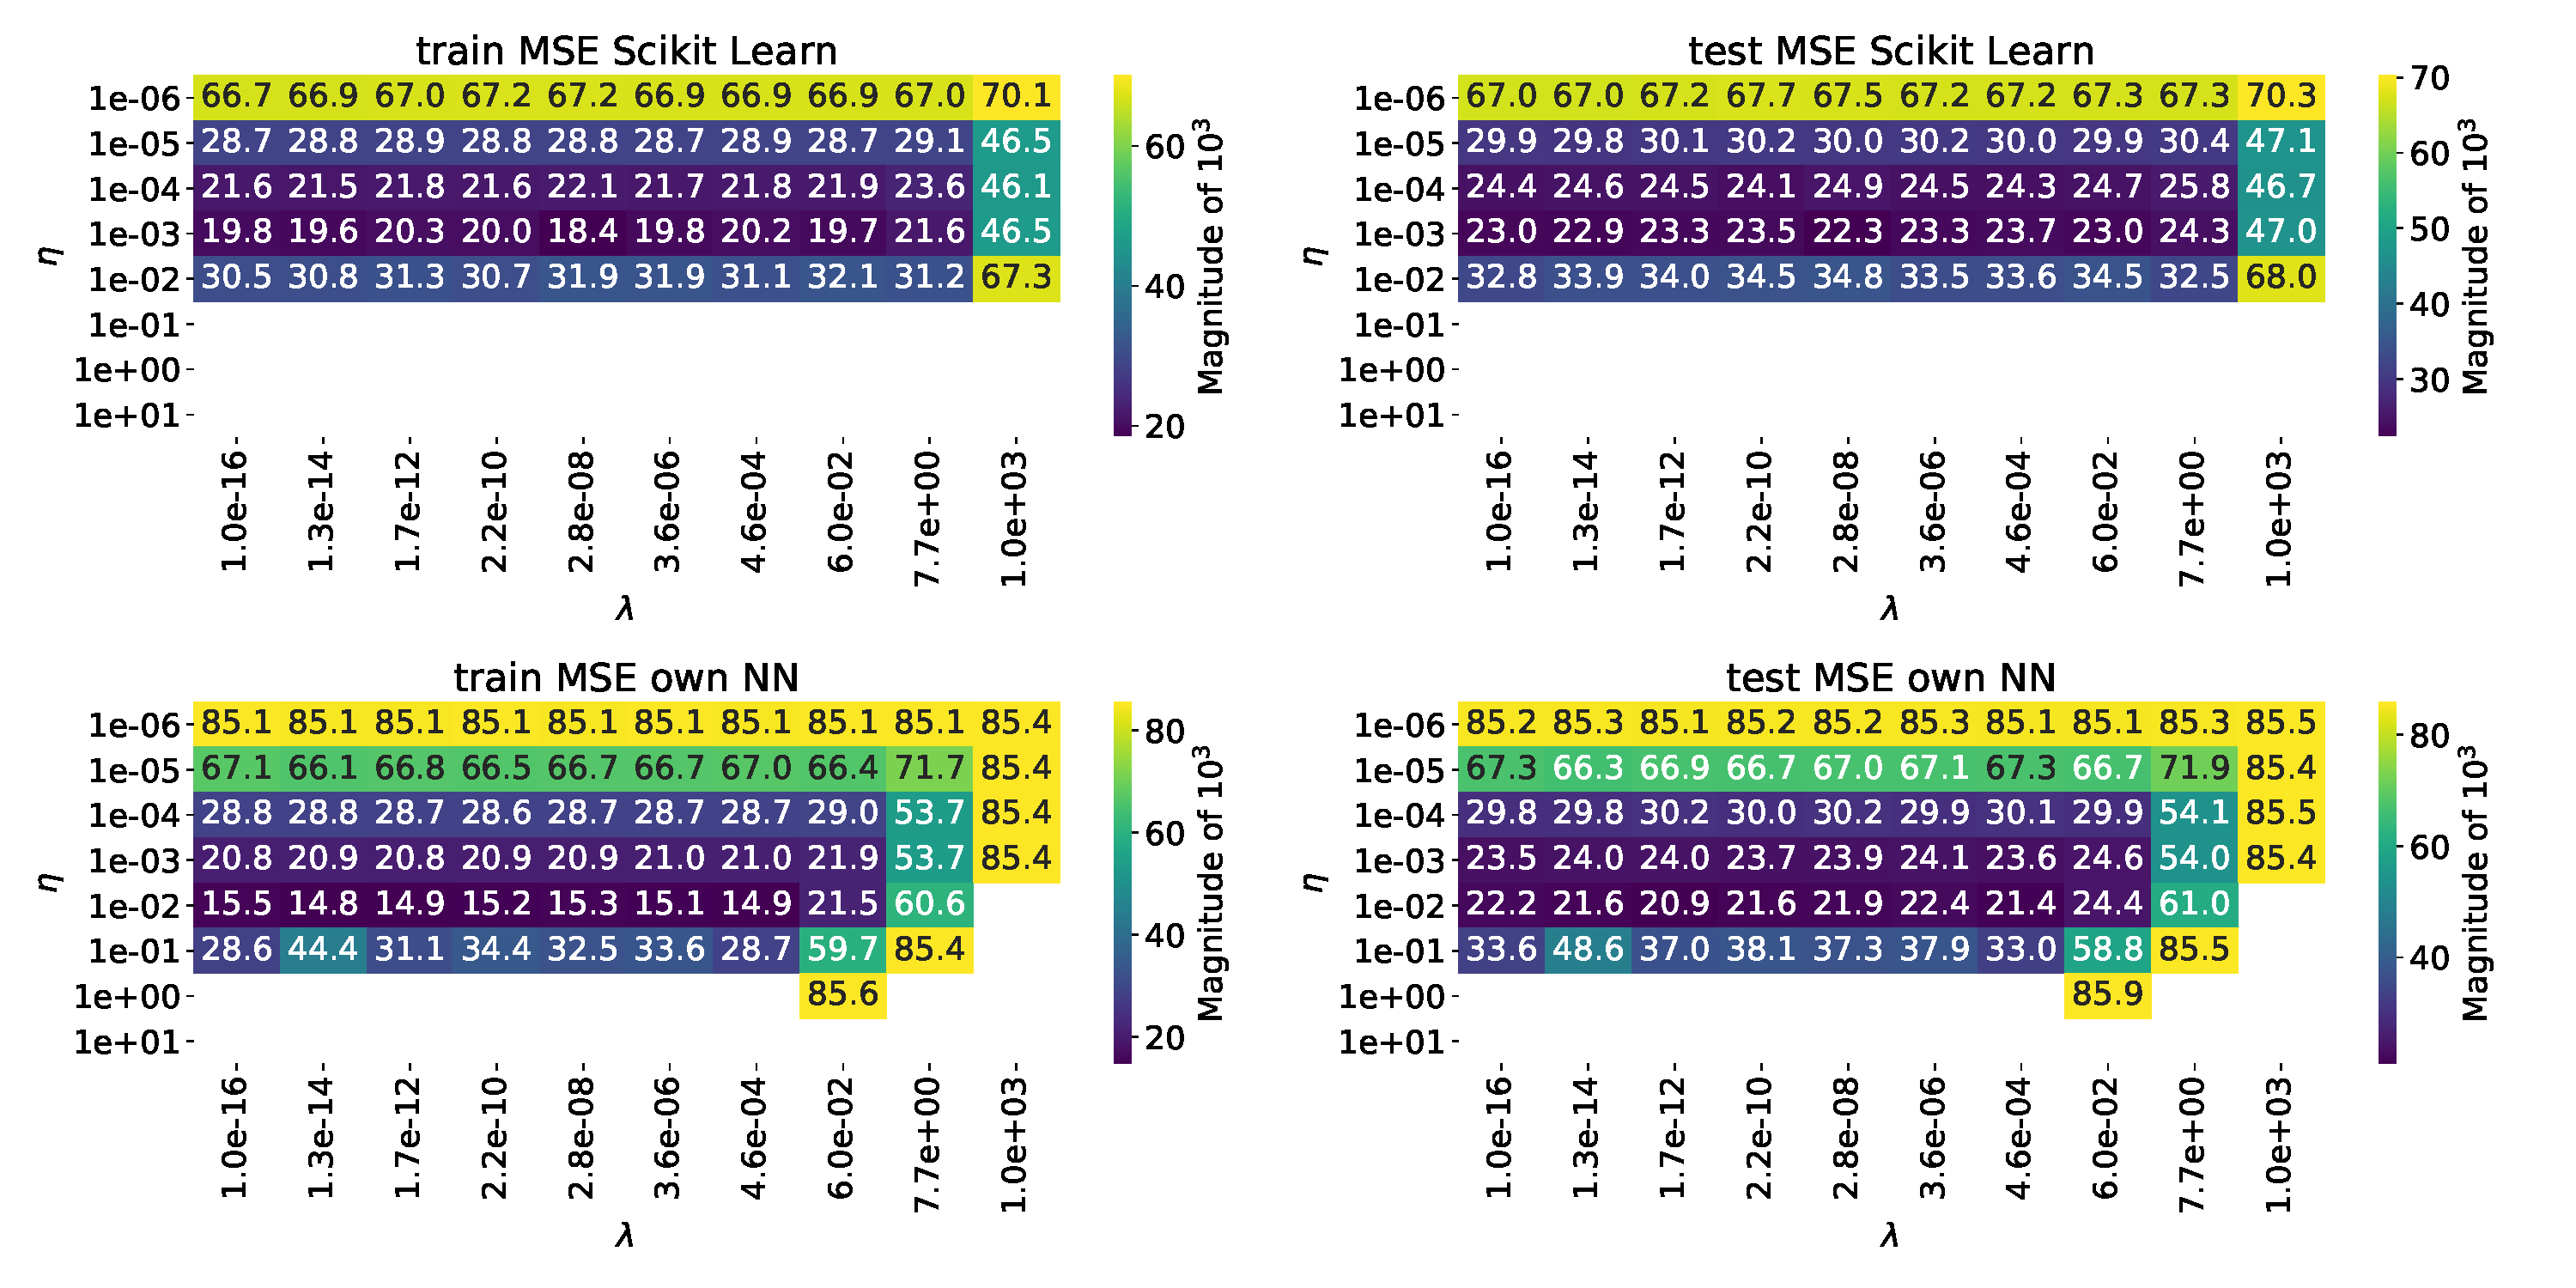
\includegraphics[width=1.05\textwidth]{scikit_own_1b1_logisticsgd200010.pdf}
\caption[Scikit-learn  and own FFNN with 1 layer]{Train and test MSE \underline{divided by 1000} as function of the learning rate $\eta$ and the regularization parameter $\lambda$ for our own Neural Network and Scikit-learn 's MLPRegressor function. We used 2000 data points (randomly selected), a polynomial degree of 10, a batch size of 200, 1000 epochs, one hidden layer with 100 neurons, simple SGD as gradient descent method and the sigmoid function as activation function between the layers. Values exceeding 100,000 are excluded from the plot. We used 5-fold Cross Validation to estimate the errors.} \label{fig:ScikitLearn_1}
\end{figure}
First of all, we see that both Scikit-learn and our own Neural Network outperform OLS (and Ridge regression, which gives identical values here). Values like that were not possible to obtain only using Linear Regression for that amount of data points \citep{Project1}, indicating that Neural Networks can give superior results to Linear Regression methods. This comes however at the cost of not obtaining a nice function expression (it is up to the reader to decide if a multivariate polynomial of degree 10 is a nice function expression - but the number of parameters is bearable) with a meaning behind it. \\
We see that our algorithm gave superior values to Scikit-learn. This is supposedly due to a different implementation of the SGD-algorithm, as is clear as the ideal parameters for the learning rate differ by one magnitude. Finally, we see that choosing wrong parameters ends up giving completely horrendous results, meaning that tweaking both the regularization parameter and the learning rate is necessary.
\subsubsection{Impact of number of hidden layers}
Exactly the same analysis as before (compare figure \ref{fig:ScikitLearn_1}) was done, this time using two hidden layers with 100 neurons each. The results can be seen in figure \ref{fig:ScikitLearn_2}.
\begin{figure}[H]
\centering
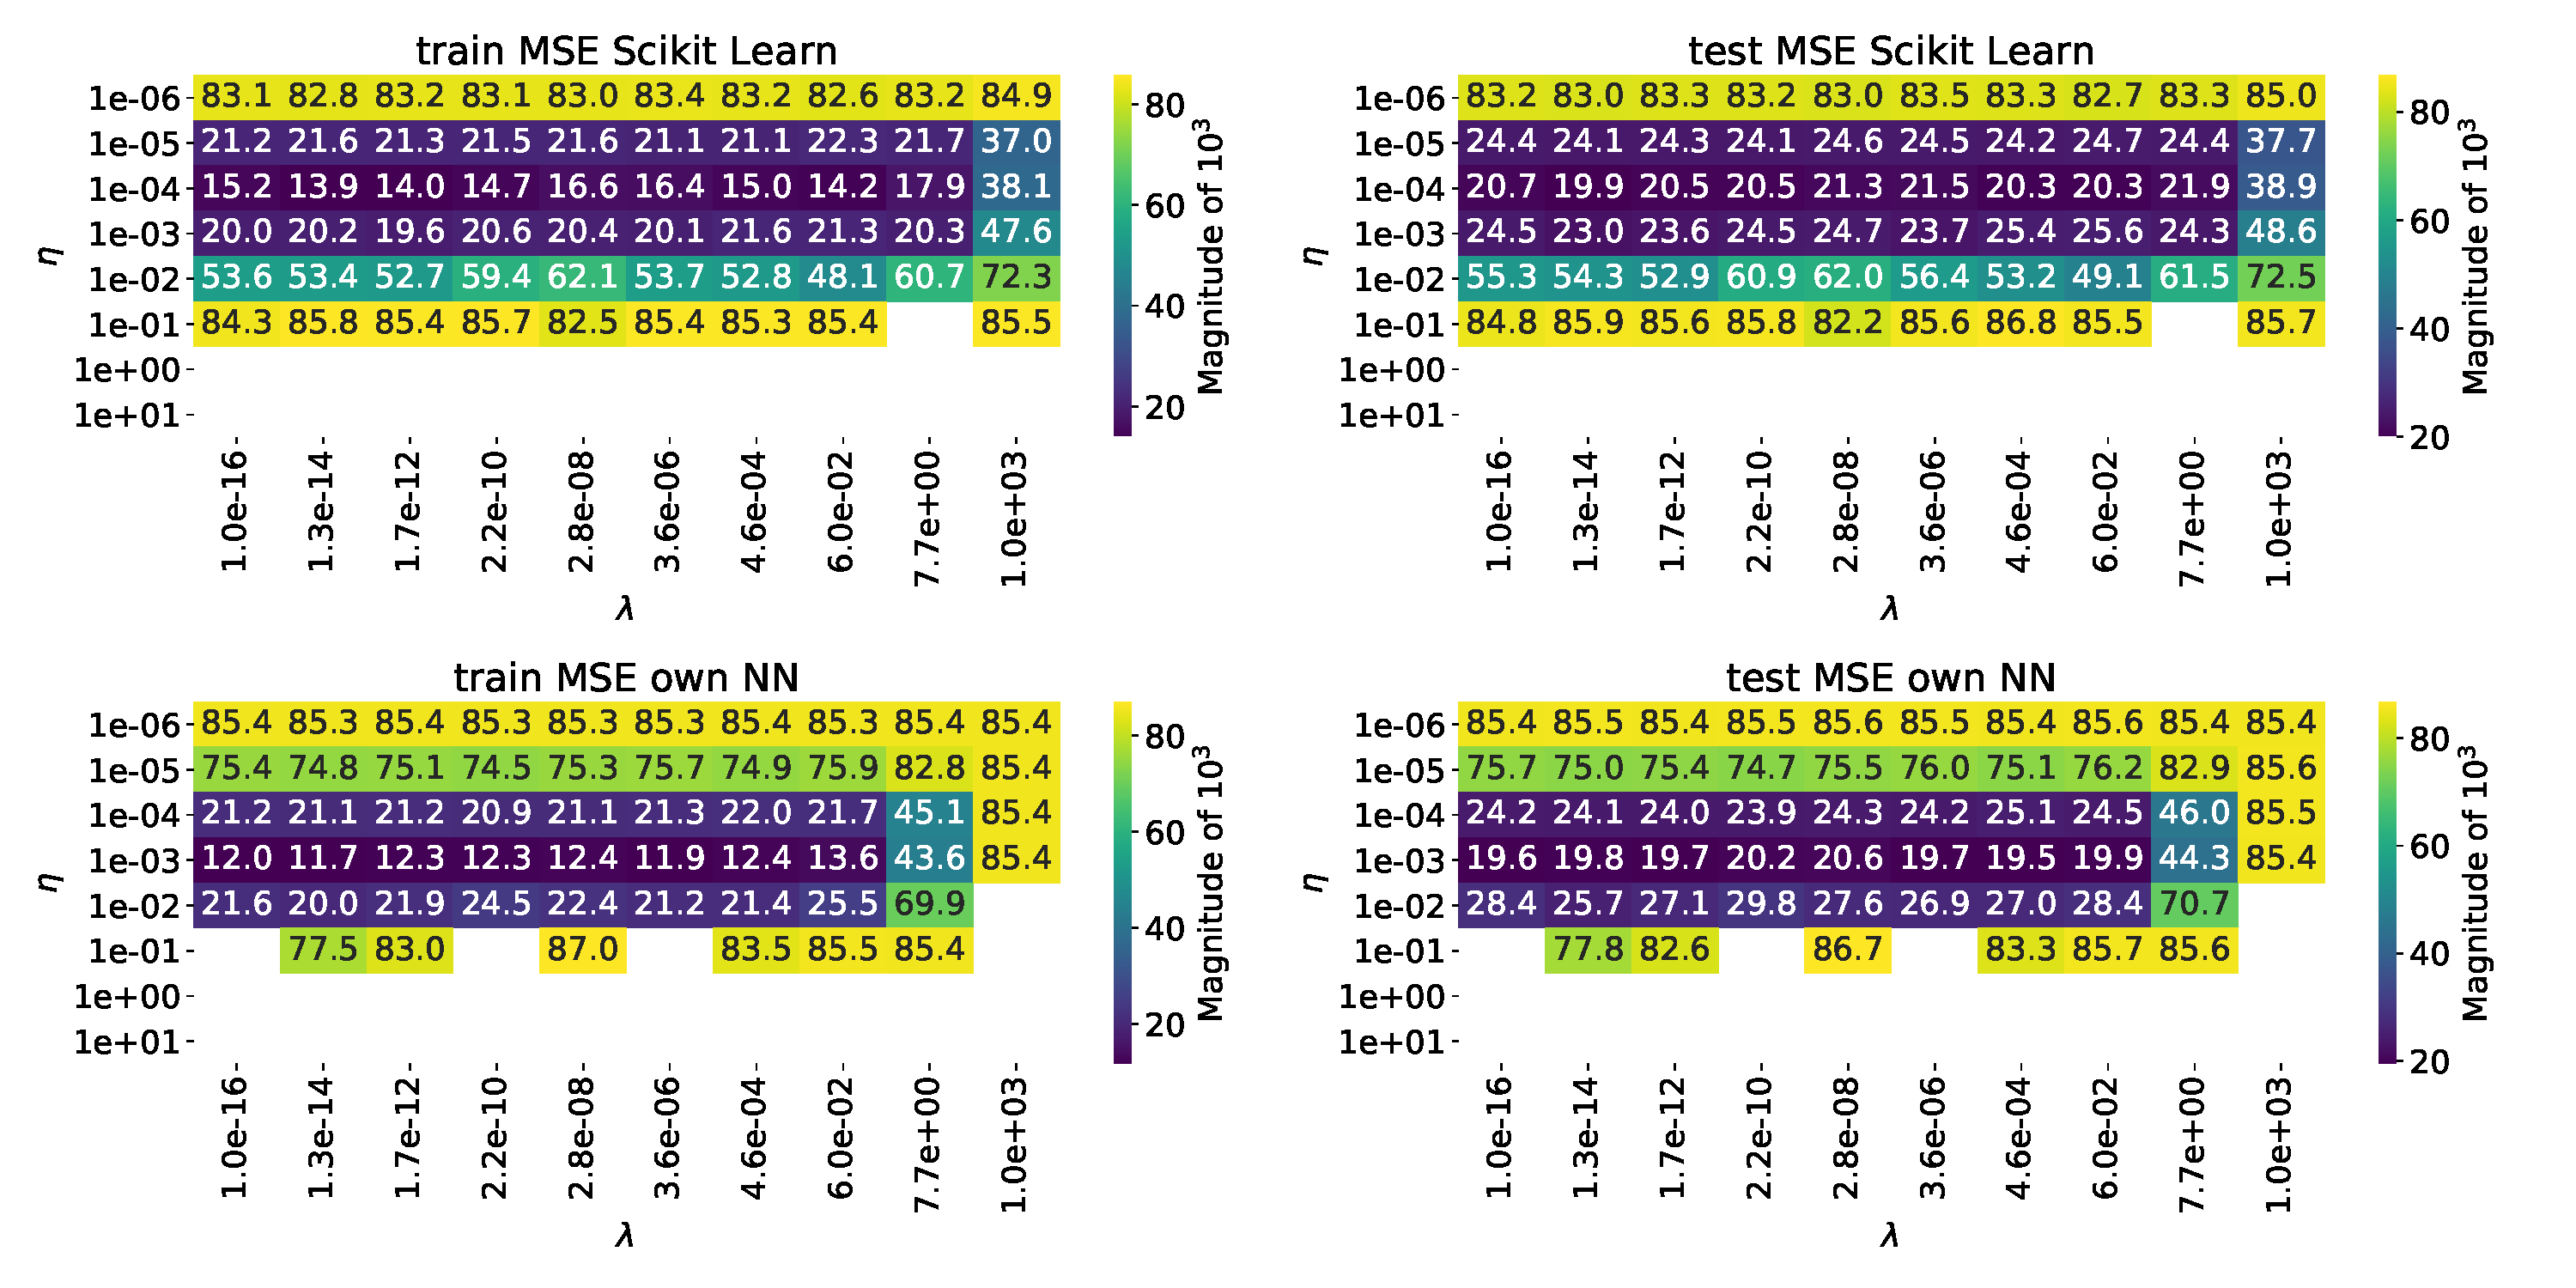
\includegraphics[width=1.05\textwidth]{scikit_own_2b1_logisticsgd200010.pdf}
\caption[Scikit-learn  and own FFNN with 2 layers]{Train and test MSE \underline{divided by 1000} as function of the learning rate $\eta$ and the regularization parameter $\lambda$ for our own Neural Network and Scikit-learn 's MLPRegressor function. We used 2000 data points (randomly selected), a polynomial degree of 10, a batch size of 200, 1000 epochs, two hidden layers with 100 neurons each, simple SGD as gradient descent method and the sigmoid function as activation function between the layers. Values exceeding 100,000 are excluded from the plot. We used 5-fold Cross Validation to estimate the errors.} \label{fig:ScikitLearn_2}
\end{figure}
We see that adding the second layer gives even better results than just using one hidden layer. This indicates that using more layers can further reduce the error. Again, our Neural Network outperforms Scikit learn, but the difference is smaller than with just one single layer.\\We also run the same analysis with a polynomial degree of 20. The results can be seen in figure \ref{fig:ScikitLearn_3} in the appendix. Here, OLS fails due to a too high variance. Ridge regression can be used though and gave a test error of 24312, while our own Neural Network with 2 layers gave a test error of 20251 (which is slightly worse than the error produced by Scikit Learn, which is 20043. The test error for the neural network has hence increased - we suppose that the increased amount of parameters leads to a slower convergence rate, it might be possible that increasing the number of iterations might lead to better parameters. 
\subsubsection{Comparison between ADAM, RMSProp \& simple SGD}
Figure \ref{fig:ADAMvsRMSProp} contains the train and the test MSE using ADAM \& RMSProp as stochastic gradient descent methods using our own FFNN. The parameters are identical to the ones in figure \ref{fig:ScikitLearn_2}, that is, two hidden layers with 100 neurons each. 
\begin{figure}[H]
\centering
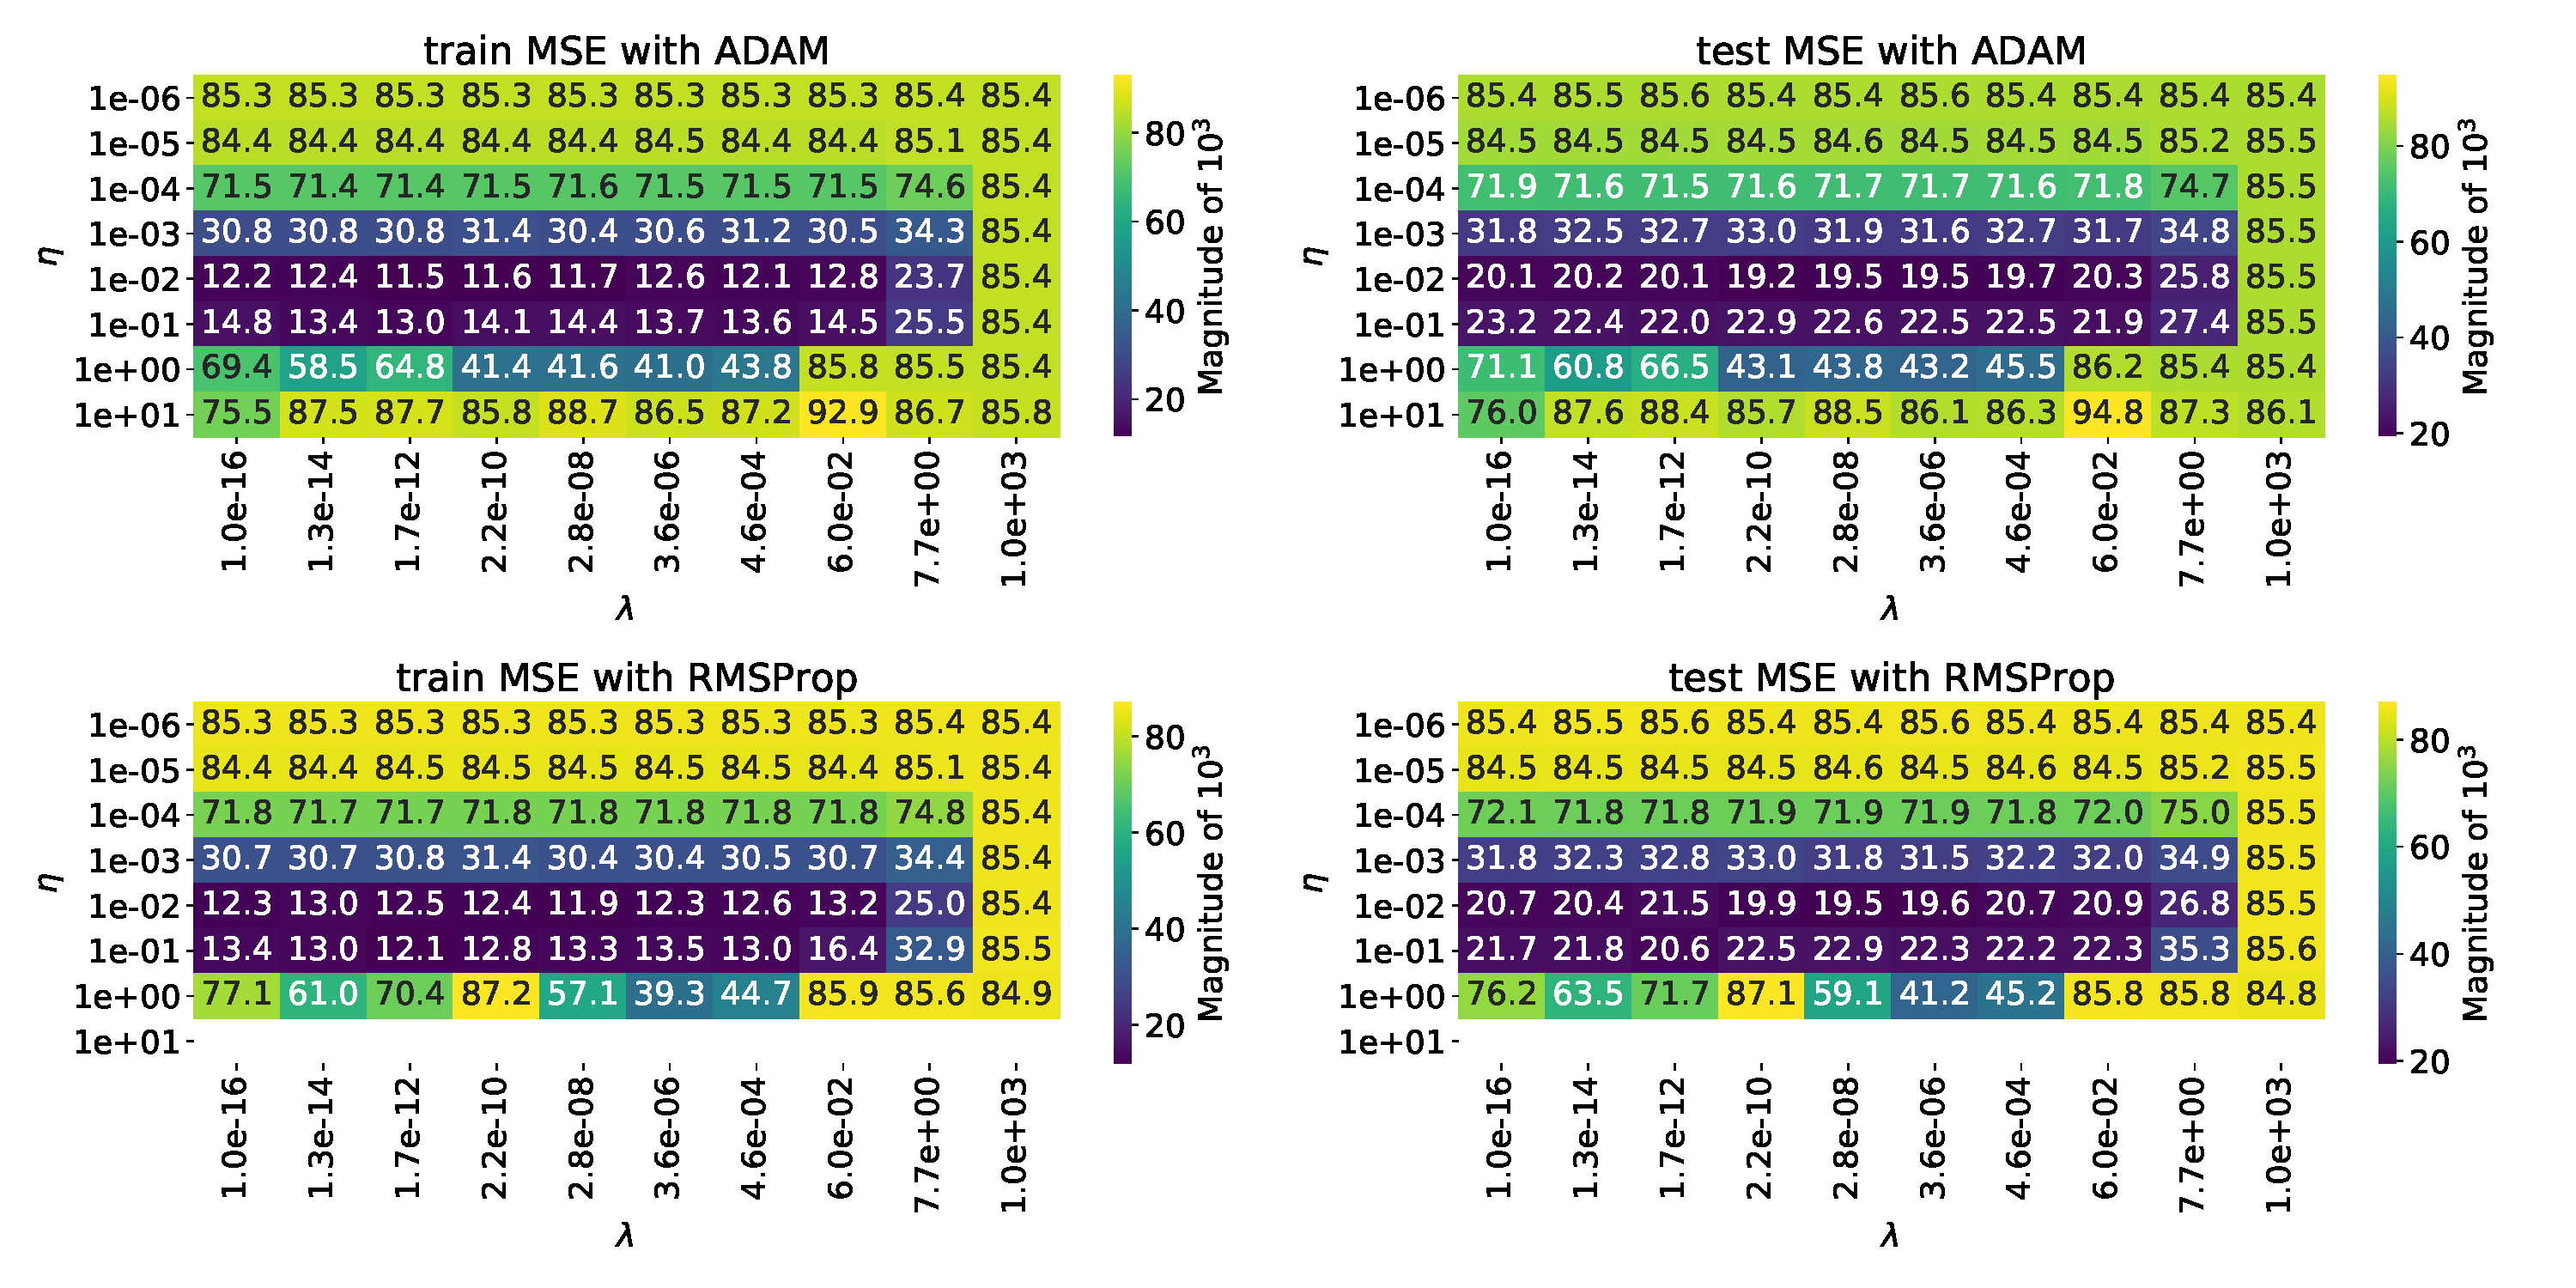
\includegraphics[width=1.05\textwidth]{ADAM_RMSProp_2b1_logisticRMSProp200010.pdf}
\caption[ADAM \& RMSProp with 2 layers]{Train and test MSE \underline{divided by 1000} as function of the learning rate $\eta$ and the regularization parameter $\lambda$ for our own Neural Network using ADAM and RMSProp. We used 2000 data points (randomly selected), a polynomial degree of 10, a batch size of 200, 1000 epochs, two hidden layers with 100 neurons each and the sigmoid function as activation function between the layers. Values exceeding 100,000 are excluded from the plot. We used 5-fold Cross Validation to estimate the errors.} \label{fig:ADAMvsRMSProp}
\end{figure}
We see that the methods are generally similar and give similar test and train errors for similar parameters. However, ADAM copes better with too high learning rates and the results at high learning rates, albeit much worse than with good parameters, do not explode. ADAM also surpasses simple SGD in the sense that the lowest obtained test MSE is slightly lower, while RMSProp is on pair. 
\subsubsection{Impact of activation function}
As ADAM has given the best test results, we used ADAM as stochastic gradient method and compared the impact of the four different activation functions ReLU, tanh, sigmoid \& LeakyReLU. This can be seen in figure \ref{fig:ADAMdifferentActivationFunctions}.
\begin{figure}[H]
\centering
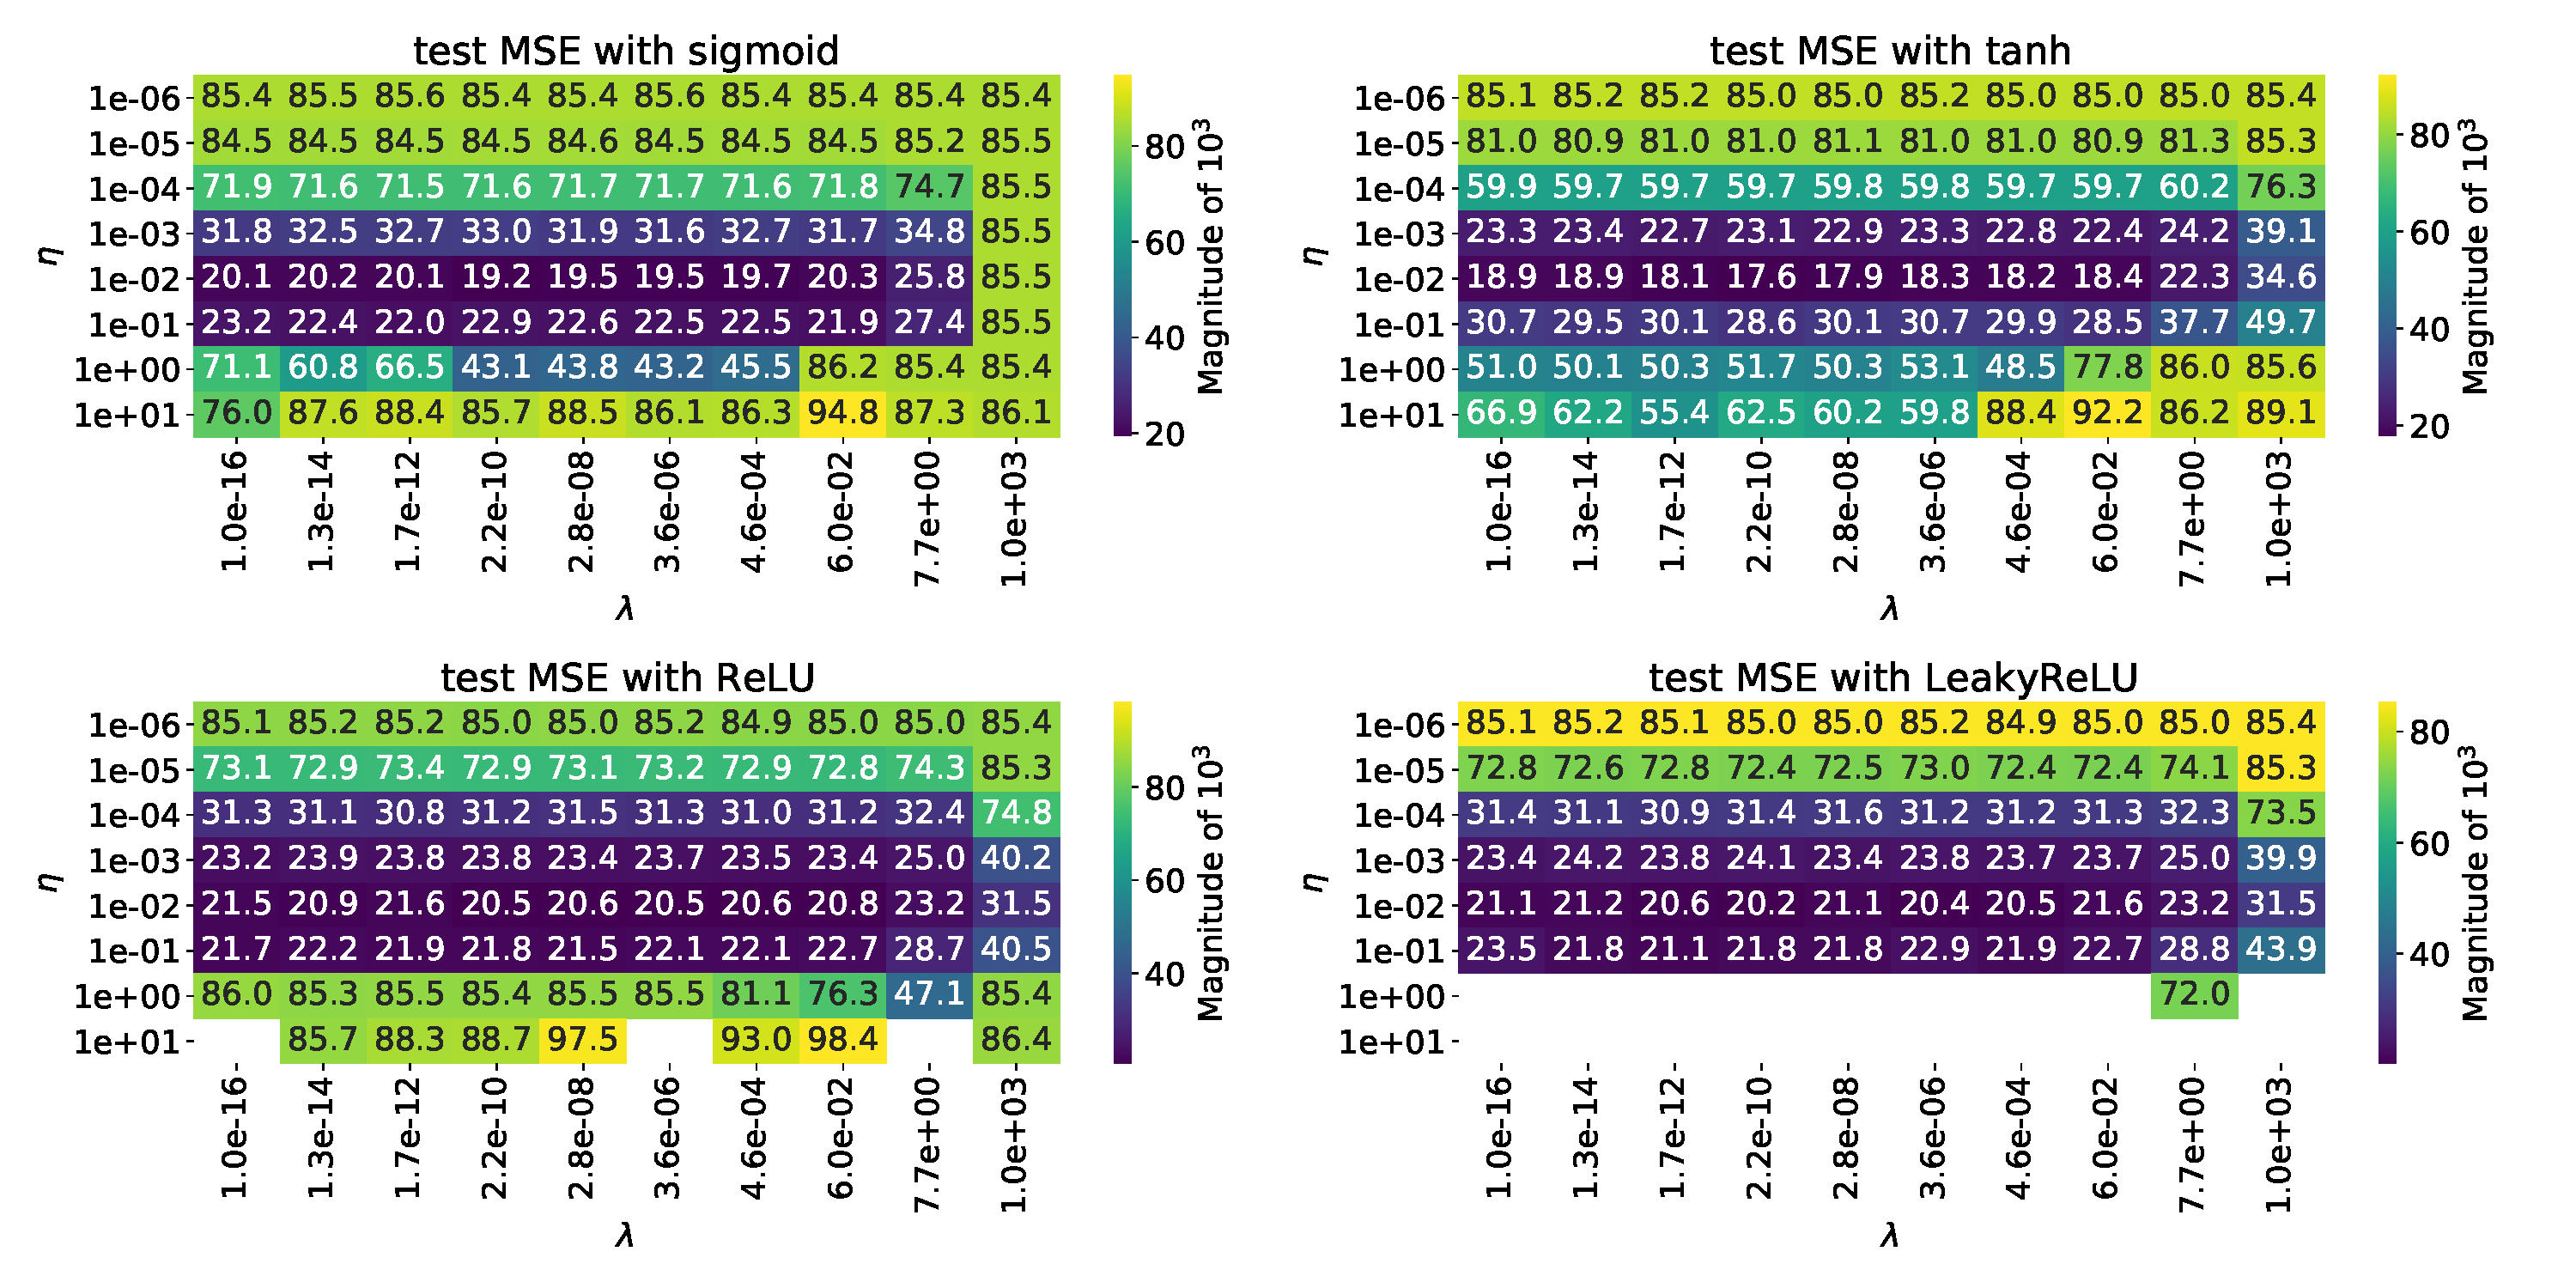
\includegraphics[width=1.05\textwidth]{Four_activations2ADAM200010.pdf}
\caption[Different activation functions]{Test MSE \underline{divided by 1000} as function of the learning rate $\eta$ and the regularization parameter $\lambda$ for our own Neural Network using ADAM. We used 2000 data points (randomly selected), a polynomial degree of 10, a batch size of 200, 1000 epochs, two hidden layers with 100 neurons each and the activation function stated in the title between the layers. Values exceeding 100,000 are excluded from the plot. We used 5-fold Cross Validation to estimate the errors.} \label{fig:ADAMdifferentActivationFunctions}
\end{figure}
As we see, the tanh function gave by far the best results with a test MSE below $18,000$, followed by the sigmoid function. This does not show that the tanh function is the best activation function, but that the tanh function in this case, with the given amount of layers and chosen parameters as well as the number of epochs, performs best. It is interesting to see that both the ReLU and the LeakyReLU activaton functions seem to be more "forgiving" to different learning rates and regularization parameters, as a larger part of the 2D table appears blue, indicating small values, than with the tanh function \& the sigmoid function.\\

For comparison, we run a small test with 4 hidden layers of sizes (100,100,50,50) (in that order, where the output layer is to the right), but only 100 epochs due to the high time usage. The result can be found in figure \ref{fig:4layers} in the appendix where the test error is portrayed for all 4 methods. From this graph, we see that ReLU \& LeakyReLU perform much better for this deeper neural network. Not only is the smallest test error lower, the methods are much more stable too, in the sense that the both ReLU and LeakyReLU give good results for much more values of the learning rate and the regularization parameter, whereas tanh and especially the sigmoid function are very narrow. Figure \ref{fig:2layers} in the appendix is also run with only 100 epochs, but has only 2 hidden layers. Here, the sigmoid function and the tanh function are superior, however the test error achieved with both the LeakyReLU and ReLU and 4 layers is lower than the test error from the tanh function and two layers (and all sigmoid function values except for one), indicating that the ReLU/LeakyReLU can indeed give better results.
\section{Conclusion}
As can be see in the preceding section on regression, getting results that surpass Ridge Regression and OLS is not difficult, which shows that neural networks are well suited for regression problems. However, finding the ideal parameters is no easy task, as there are a lot of activation functions, gradient methods and parameters to choose. There is also the aspect of time - higher epochs lead to superior results, but the error reduces extremely slow as the number of epochs grows exponentially \citep{handsOnMachineLearning}. For the regression problem, we found, with help of the sigmoid function, that ADAM worked best as stochastic gradient method, whereas the tanh activation function worked best as activation function (with 2 hidden layers), giving $60\%$ of the test MSE that OLS produces. However, as the network got deeper, we found that...XXX blablabla
\section{Appendix}
\subsection{Proof that Softmax reduces to the Logistic function for m=2}\label{ProofSoftmaxToLogistic}

Consider the Softmax function for $m=2$ categories

\begin{equation}
\textbf{a} = \frac{1}{ \exp(\textbf{W}_{[1,:]}\cdot \textbf{x}^T)  + \exp( \textbf{W}_{[2,:]} \cdot \textbf{x}^T ) }
\begin{pmatrix}
\exp( \textbf{W}_{[1,:]} \cdot \textbf{x}^T) \\
\exp( \textbf{W}_{[2,:]} \cdot \textbf{x}^T)
\end{pmatrix}
\end{equation}
We can multiply both sides of the fraction by $\exp(- \textbf{W}_{[2,:]} \cdot \textbf{x}^T)$ to get
\begin{equation}
\textbf{a} = \frac{1}{ 1  + \exp( (\textbf{W}_{[1,:]} -\textbf{W}_{[2,:]})\cdot \textbf{x}^T) }
\begin{pmatrix}
\exp( (\textbf{W}_{[1,:]} -\textbf{W}_{[2,:]})\cdot \textbf{x}^T) \\
\exp( \vec{0})
\end{pmatrix}
\end{equation}
We can now simply rename this weight parameter as $\textbf{W}_{[1,:]} -\textbf{W}_{[2,:]} = -\textbf{W}$ giving us
\begin{equation}
a = \begin{pmatrix}
\frac{\exp( -\textbf{W}\cdot \textbf{x}^T)}{1+\exp( -\textbf{W}\cdot \textbf{x}^T)} \\
\frac{1}{1+ \exp( -\textbf{W}\cdot \textbf{x}^T)}
\end{pmatrix} = \begin{pmatrix}
1-\frac{1}{1+\exp( -\textbf{W}\cdot \textbf{x}^T)} \\
\frac{1}{1+ \exp( -\textbf{W}\cdot \textbf{x}^T)}
\end{pmatrix} 
\end{equation}
which is the same as the activation function for logistic regression.
\begin{figure}[H]
\centering
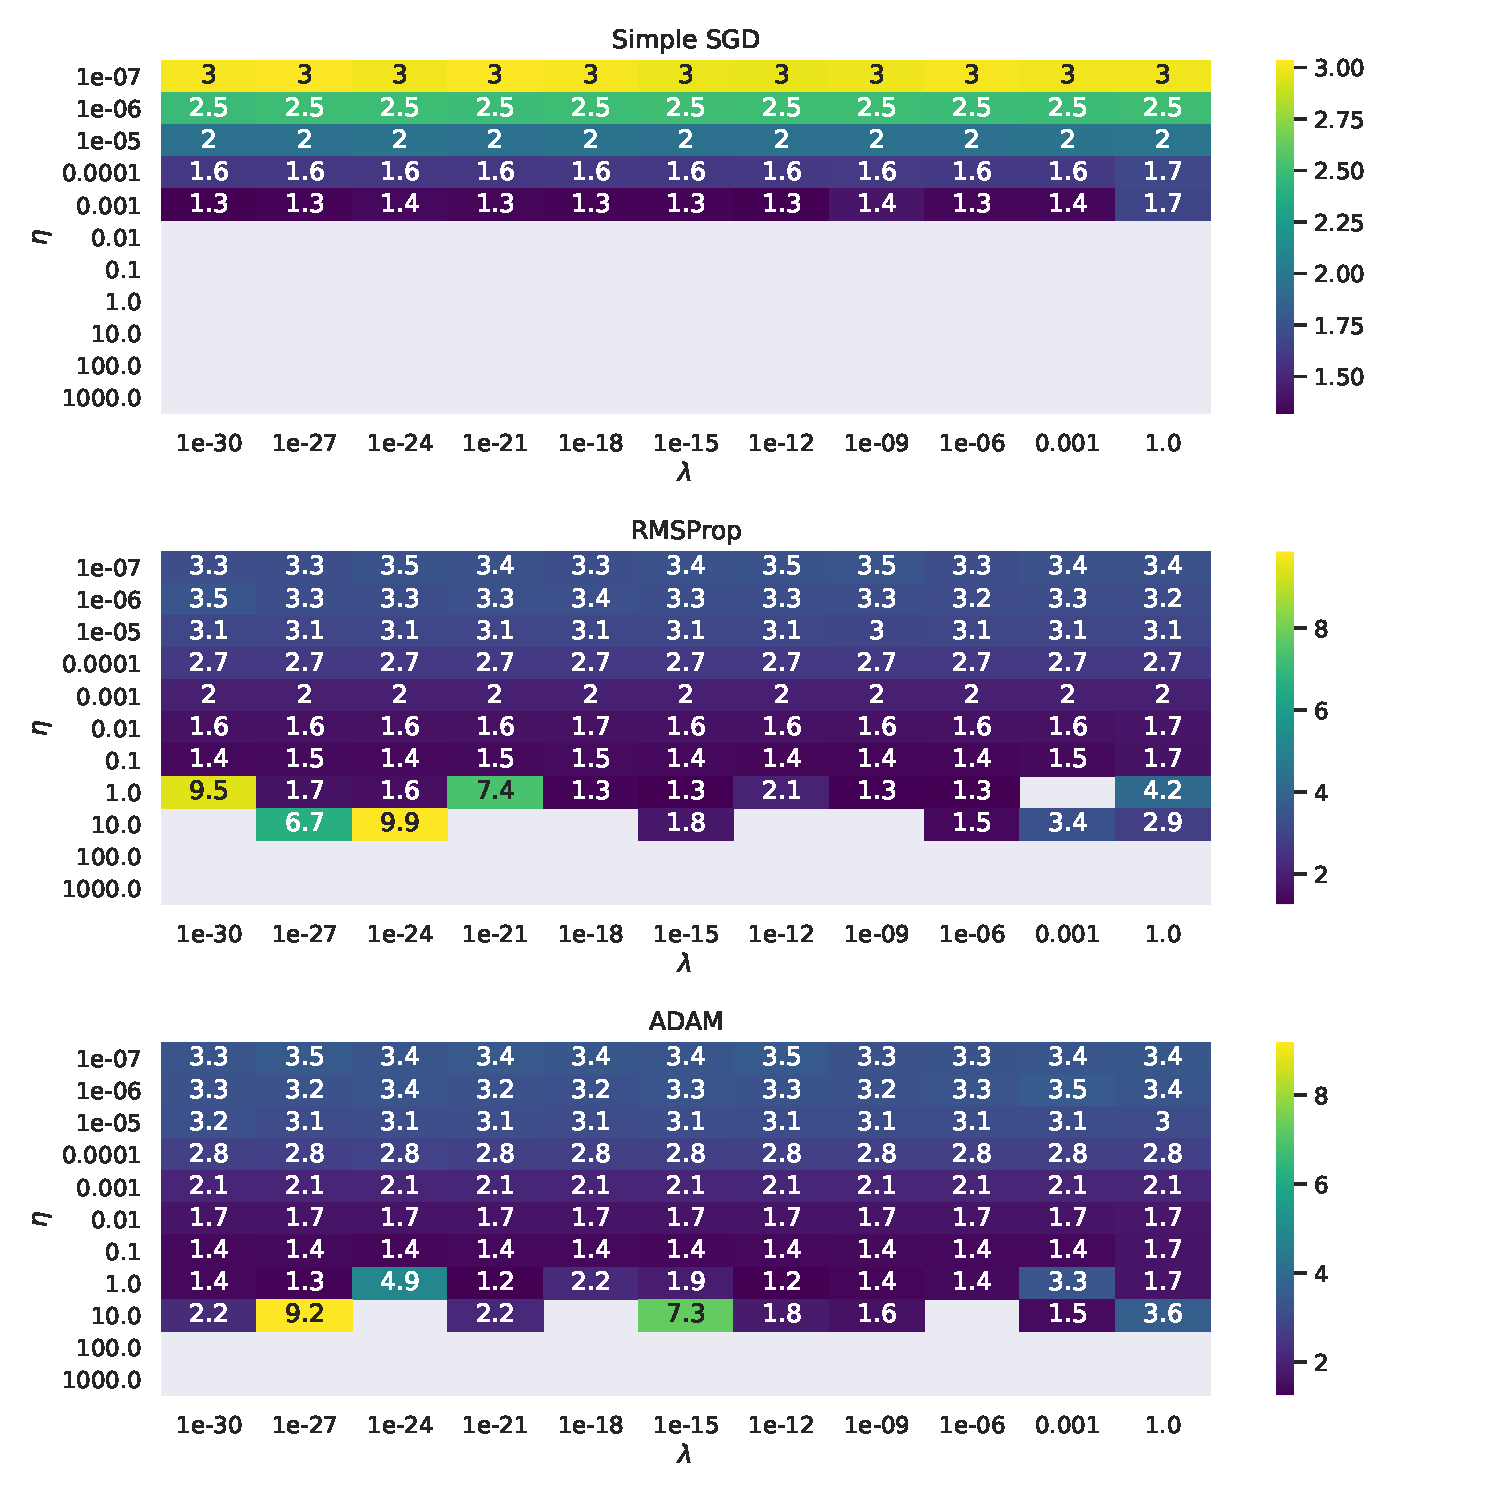
\includegraphics[width=0.95\textwidth]{Ridge_error_SGD.pdf}
\caption[Relative Test MSE with different SGD methods for Ridge]{Relative Test MSE  ($\frac{MSE_{SGD}}{MSE_{analytical}})$ for the simple SGD method, RMSProp and ADAM and as functions of the learning rate $\eta$ and the regularization parameter $\lambda$. $N=2000$, the polynomial degree used is $deg=20$, where OLS fails. The batch size is 16, the number of epochs is 1000. Values exceeding 10 were removed, explaning the grey parts. No bootstrapping or cross-validation was performed.} \label{fig:DifferentSGDRIDE}
\end{figure}

\begin{figure}[H]
\centering
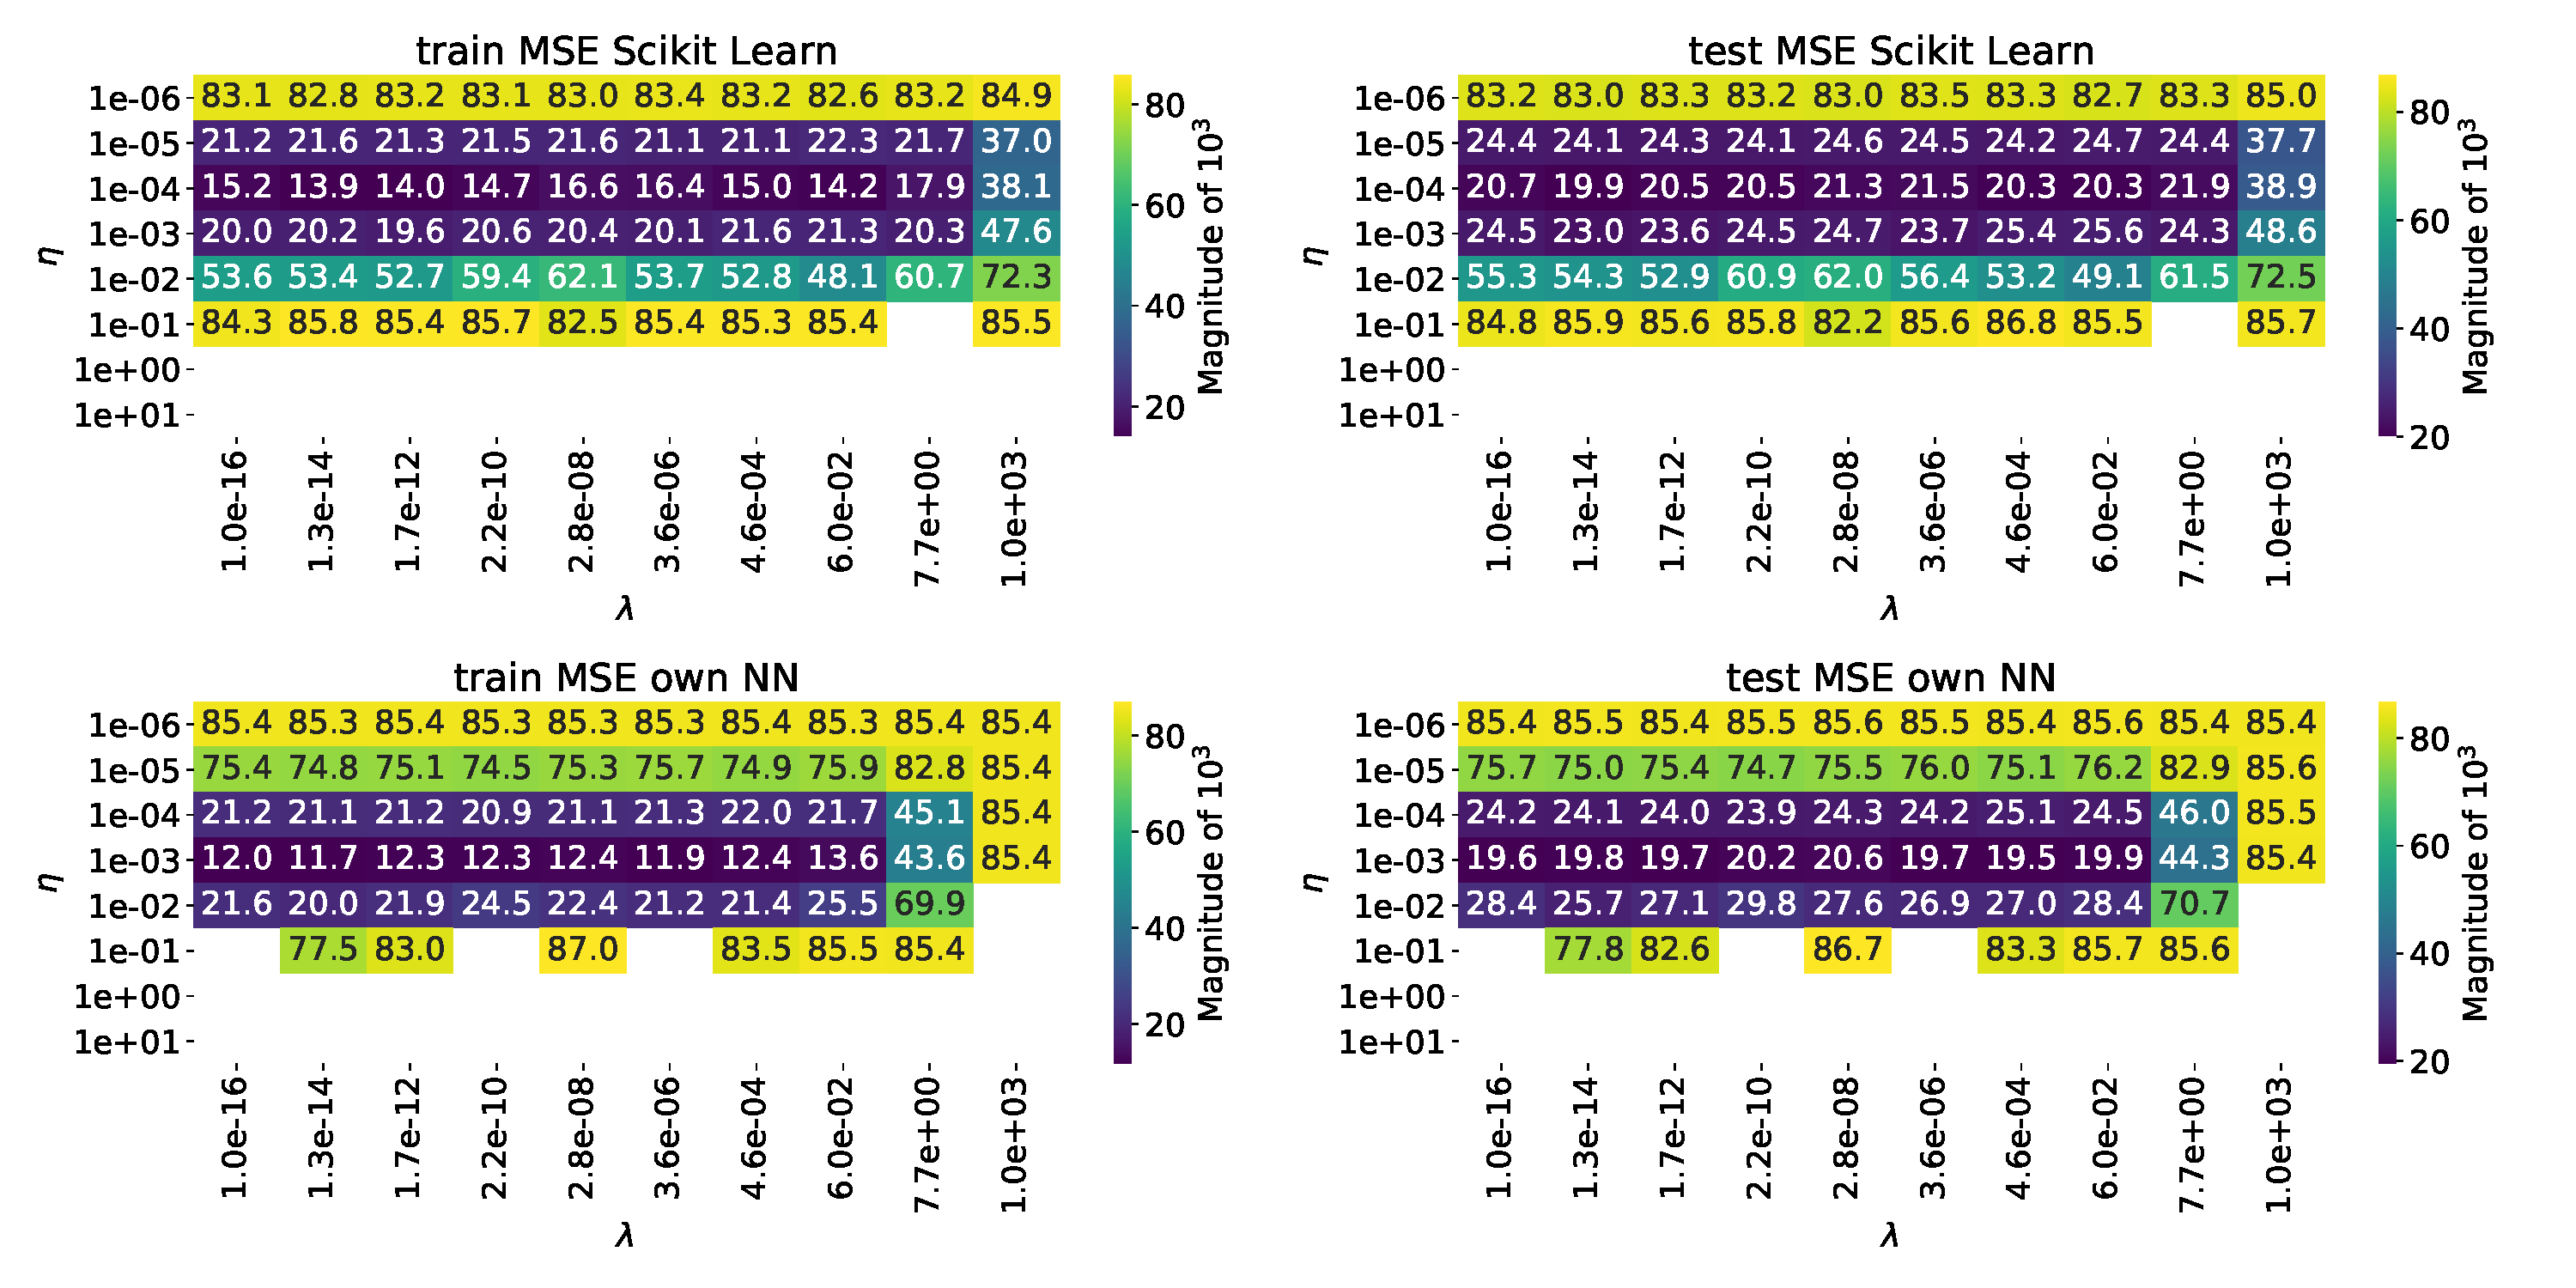
\includegraphics[width=1.05\textwidth]{scikit_own_2b1_logisticsgd200010.pdf}
\caption[Scikit-learn  and own FFNN with 2 layers, degree 20]{Train and test MSE \underline{divided by 1000} as function of the learning rate $\eta$ and the regularization parameter $\lambda$ for our own Neural Network and Scikit-learn 's MLPRegressor function. We used 2000 data points (randomly selected), a polynomial degree of 20, a batch size of 200, 1000 epochs, two hidden layers with 100 neurons each, simple SGD as gradient descent method and the sigmoid function as activation function between the layers. Values exceeding 100,000 are excluded from the plot. We used 5-fold Cross Validation to estimate the errors.} \label{fig:ScikitLearn_3}
\end{figure}
\begin{figure}[H]
\centering
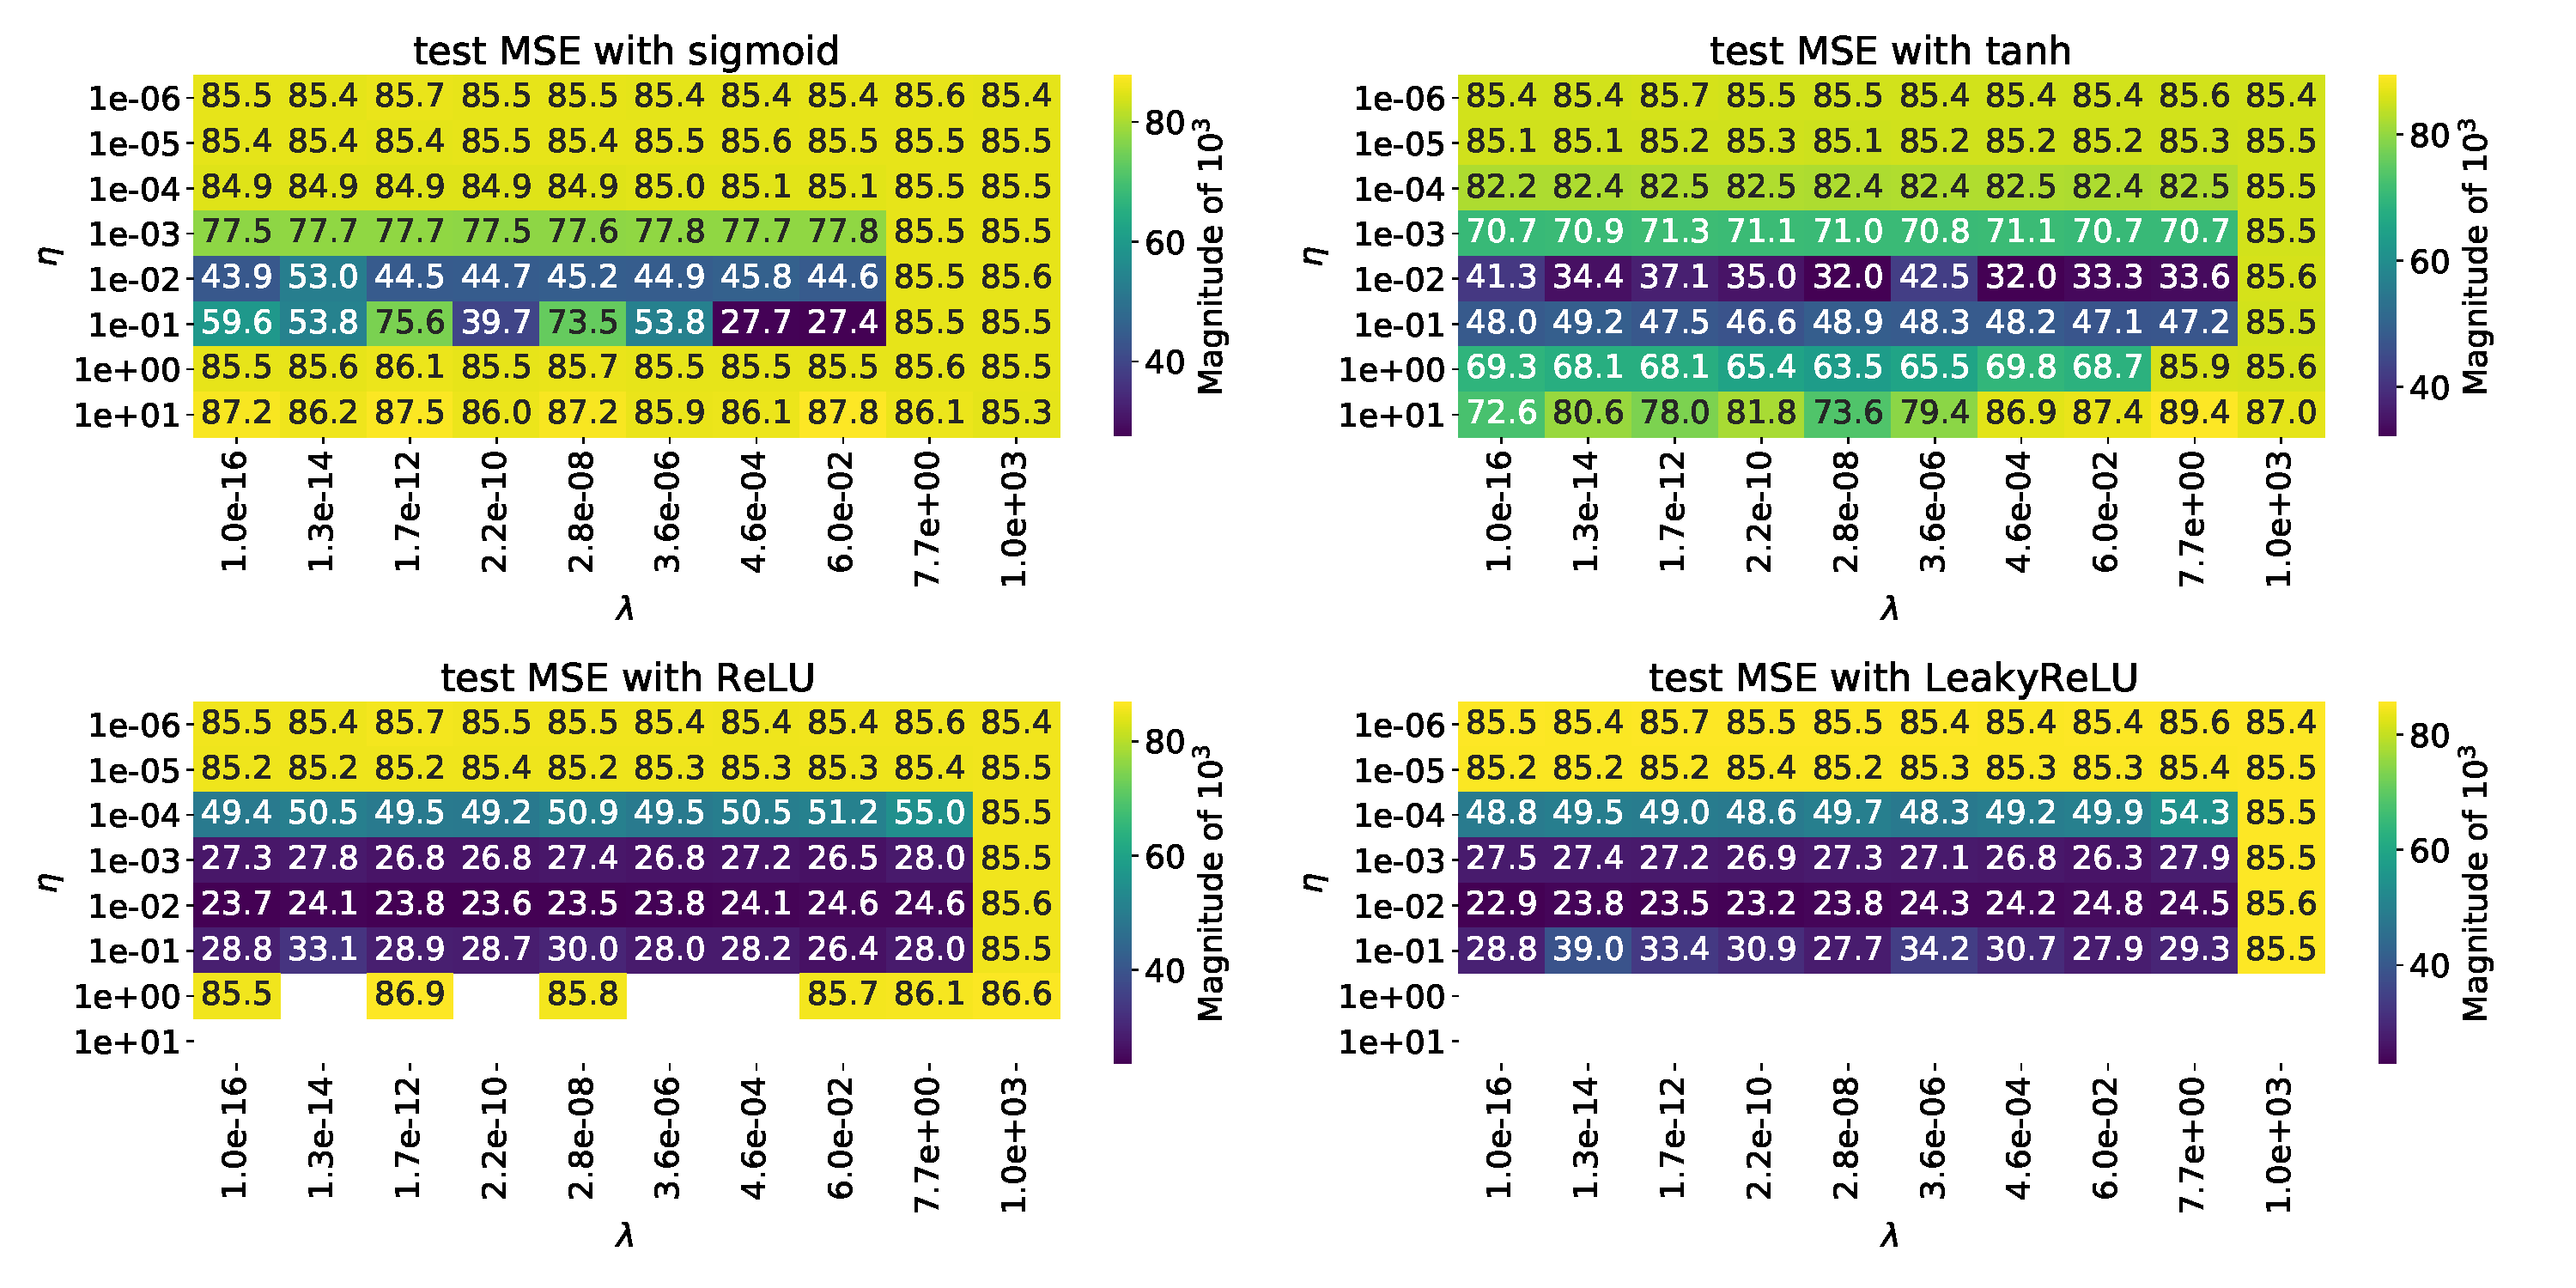
\includegraphics[width=1.0\textwidth]{4_layers.pdf}
\caption[4 hidden layers, 100 epochs]{Test MSE \underline{divided by 1000} as function of the learning rate $\eta$ and the regularization parameter $\lambda$ for our own Neural Network using ADAM. We used 2000 data points (randomly selected), a polynomial degree of 10, a batch size of 200, 1000 epochs, 4 hidden layers with respectively 100, 100, 50 and 50 neurons and the activation function stated in the title between the layers. Values exceeding 100,000 are excluded from the plot. We used 5-fold Cross Validation to estimate the errors.} \label{fig:4layers}
\end{figure}
\begin{figure}[H]
\centering
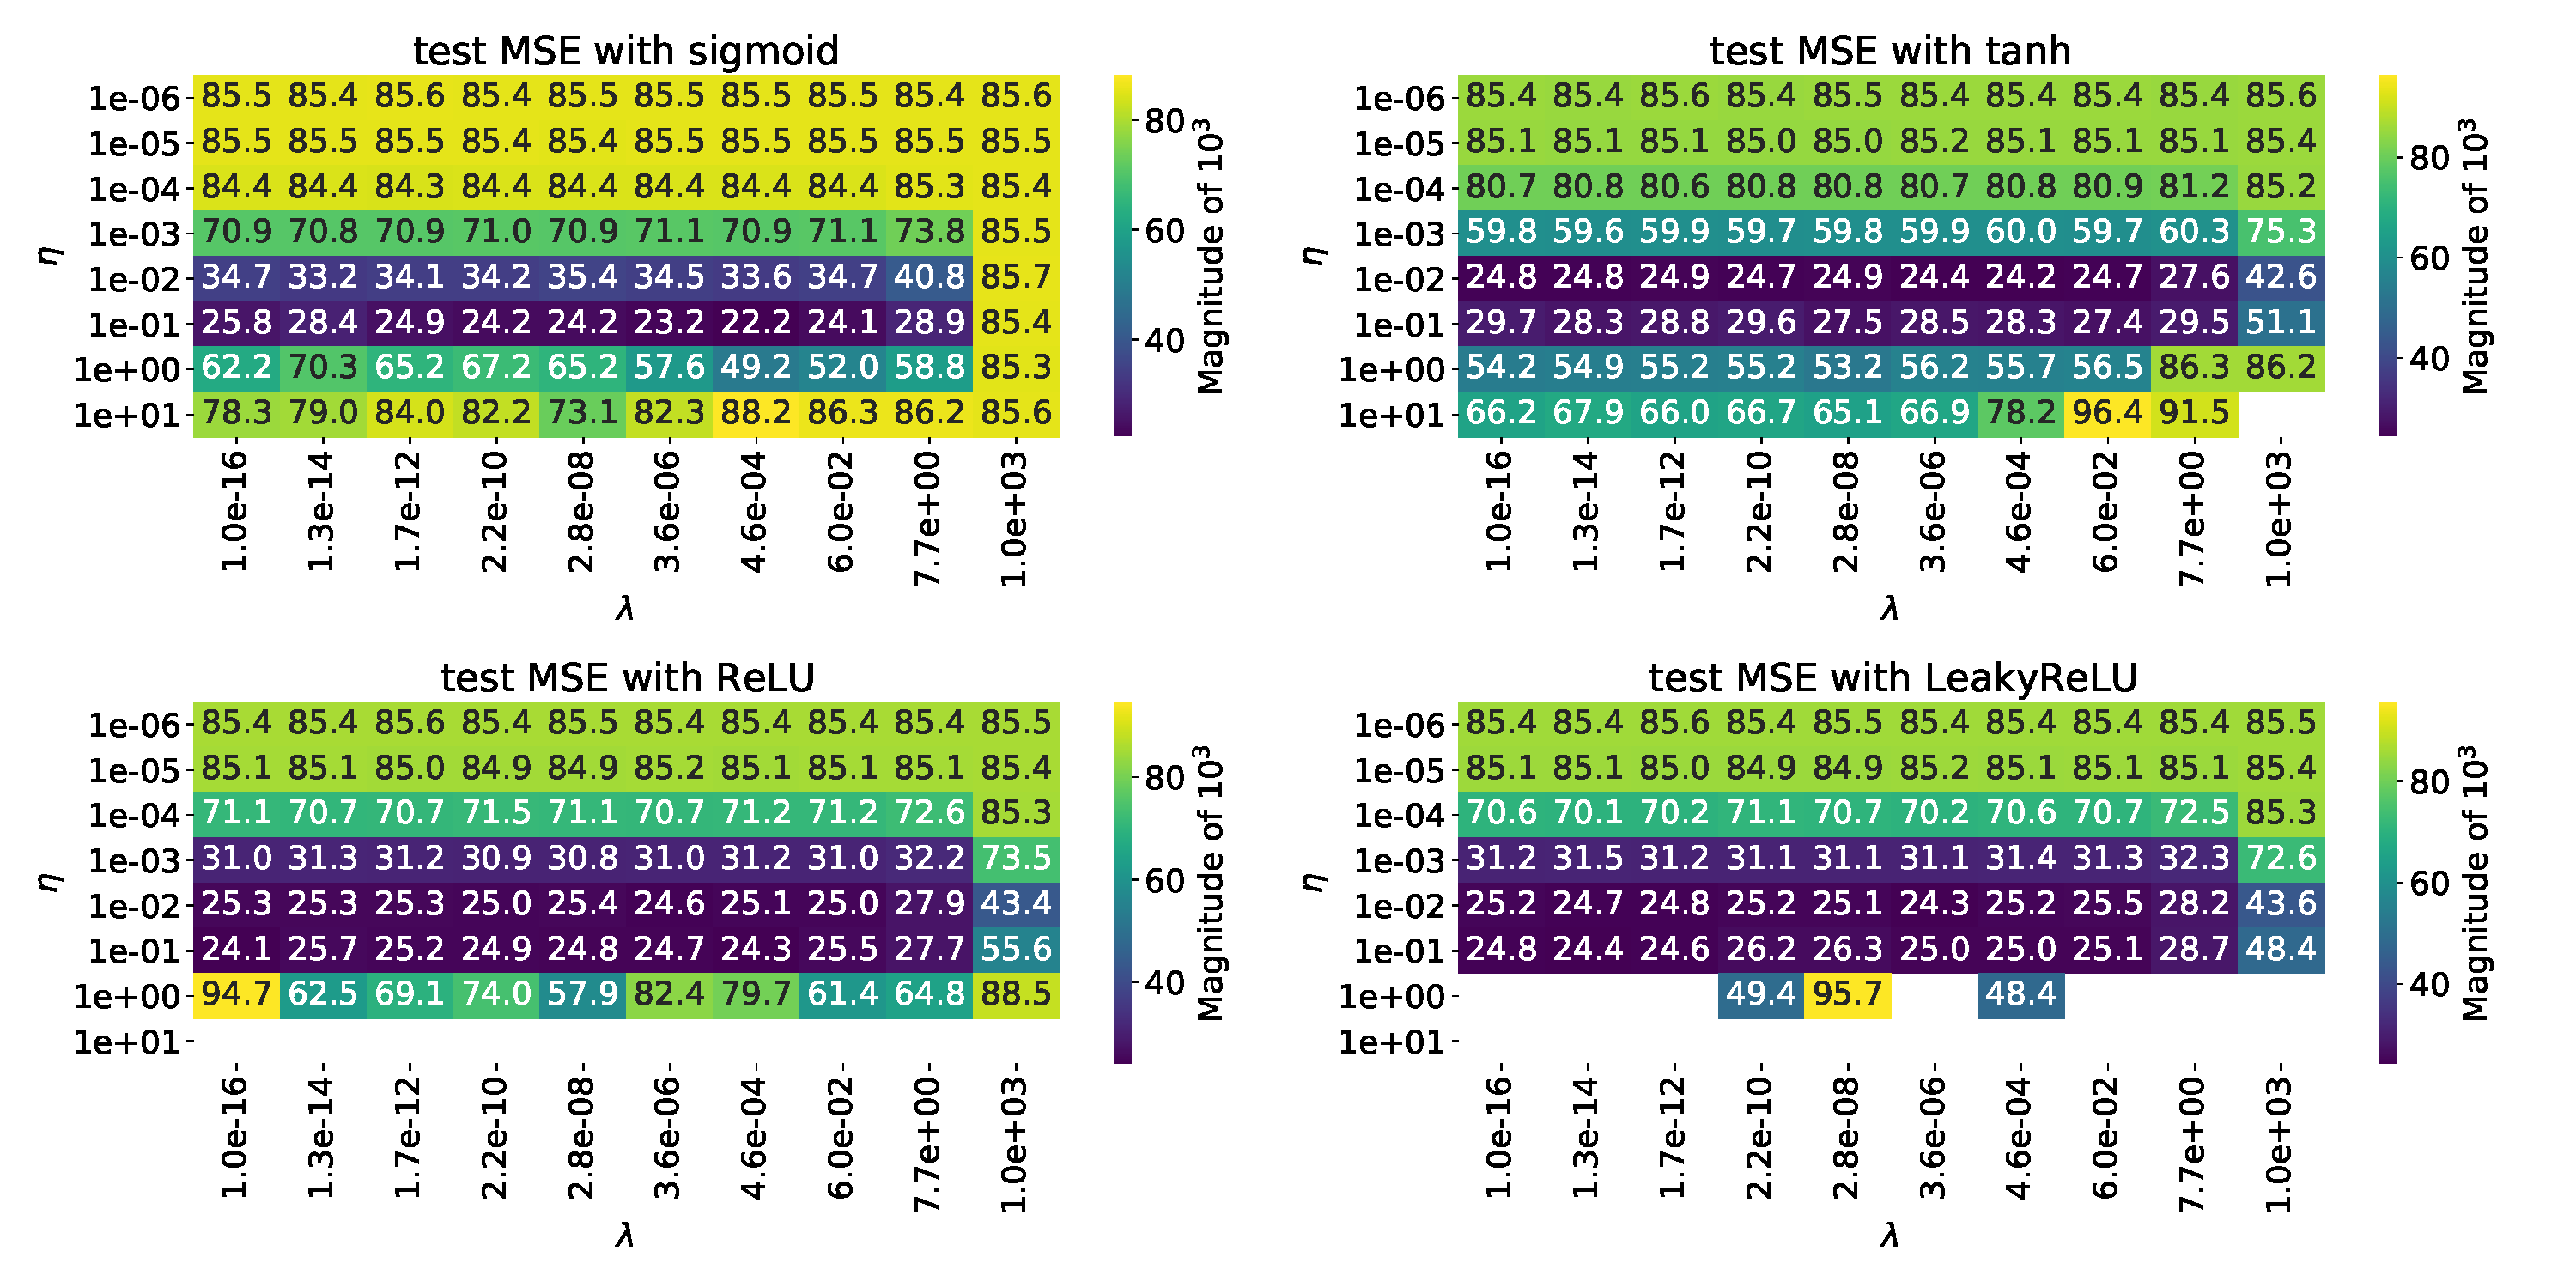
\includegraphics[width=1.0\textwidth]{2_layers_short.pdf}
\caption[4 hidden layers, 100 epochs]{Test MSE \underline{divided by 1000} as function of the learning rate $\eta$ and the regularization parameter $\lambda$ for our own Neural Network using ADAM. We used 2000 data points (randomly selected), a polynomial degree of 10, a batch size of 200, 100 epochs, two hidden layers with 100 neurons each and the activation function stated in the title between the layers. Values exceeding 100,000 are excluded from the plot. We used 5-fold Cross Validation to estimate the errors.} \label{fig:2layers}
\end{figure}

\subsection{Figures}
\bibliographystyle{plain}
\bibliography{references}
\end{document}
